\documentclass[final,leqno]{siamltex1213}
\usepackage{amsmath,amssymb}
%\usepackage{geometry} % see geometry.pdf on how to lay out the page. There's lots.
%\geometry{a4paper} % or letter or a5paper or ... etc
% \geometry{landscape} % rotated page geometry

%  POSSIBLY USEFULE PACKAGES
\usepackage{graphicx}
\usepackage{caption,subcaption}
\usepackage{tensor}
\usepackage[boxed,ruled]{algorithm2e}
\usepackage{todonotes}

%  NEW COMMANDS
\newcommand{\ram}[1]{{\normalsize{\textbf{({\color{red}RAMBO:\ }#1)}}}}
\newcommand{\hoj}[1]{{\normalsize{\textbf{({\color{blue}HOJ:\ }#1)}}}}
\newcommand{\pder}[2]{\ensuremath{\frac{ \partial #1}{\partial #2}}}
\newcommand{\ppder}[3]{\ensuremath{\frac{\partial^2 #1}{\partial{align}
      #2 \partial #3} } }

%  NEW THEOREM ENVIRONMENTS
\newtheorem{example}[theorem]{Example}
\newtheorem{ass}[theorem]{Assumption}

% NEW ENVIRONMENTS

%  MATH OPERATORS
\DeclareMathOperator{\Diff}{Diff}
\DeclareMathOperator{\Dens}{Dens}
\DeclareMathOperator{\U}{U}
\DeclareMathOperator{\OdeSolve}{OdeSolve}
\DeclareMathOperator{\Tr}{Tr}

%  TITLE, AUTHOR, DATE
\title{Qualitatively accurate spectral schemes for advection and transport}
\author{Henry O. Jacobs \& Ram Vasudevan}
\date{\today}


\begin{document}

\maketitle

\begin{abstract}
	The transport and continuum equations exhibit a number of conservation laws.
	For example, scalar multiplication is conserved by the transport equation, while
	positivity of probabilities is conserved by the continuum equation.
	Certain discretization techniques, such as particle based methods, conserve these properties, but converge slower than spectral discretization methods on smooth data.
	Standard spectral discretization methods, on the other hand, do not conserve the invariants of the transport equation and the continuum equation.
	This article constructs a novel spectral discretization technique that conserves these important invariants while simultaneously preserving spectral convergence rates. 
\end{abstract}

%%%%%%%%%%%%%%%%%%%%%%%%%%%%%%%%%%%%%%%%%%%%%%%%%%%
\section{Introduction}
\label{sec:intro}

Let $M$ be a compact $n$-manifold with local coordinates $x^{1},\dots,x^{n}$
and let $X$ be a smooth vector-field on $M$, whose local components are given by $(X^{1}(x), \dots, X^{n}(x) )$. 
This paper is concerned with the following pair of partial differential equations (PDEs):
\begin{align}
	\partial_{t} f + X^{i} \partial_{i} f = 0 \label{eq:function pde} \\
	\partial_{t} \rho + \partial_{i} (\rho X^{i}) = 0 \label{eq:density pde}
\end{align}
for a time dependent function $f$ and a time dependent density $\rho$ on $M$.
In the above PDEs we are following the Einstein summation convention, and summing over the dummy index ``$i$''.
Equation \eqref{eq:function pde}, which is sometimes called the ``transport equation,'' describes how a scalar quantity is transported by the flow of $X$ \cite{Truesdell1991}.
Equation \eqref{eq:density pde}, which is sometimes called the ``continuum equation'' or ``Liouville's equation'' describes how a density (e.g. a probability distribution) is transported by the flow of $X$.
Such PDEs arises in a variety of contexts, ranging from  mechanics \cite{Batchelor1999,Truesdell1991} to control theory \cite{HenrionKorda2014}, and can be seen as zero-noise limits of the forward and backward Kolmogorov equations \cite{Oksendal2003}.

The solution to \eqref{eq:function pde} takes the form $f(x;t) = f( (\Phi_{X}^{t})^{-1}(x) ; 0) \equiv (\Phi_{X}^{t})_{*} f(\cdot;0)$
where $\Phi_{X}^{t}:M \to M$ is the flow map of $X$ at time $t$ \cite[Chapter 18]{Lee2006}.
From this we see that \eqref{eq:function pde} exhibits a variety of conservation laws.
For example, if $f$ and $g$ are solutions to \eqref{eq:function pde},
then so is their product, $f \cdot g$, and their sum, $f+g$.
Similarly, the solution to \eqref{eq:density pde} takes the form $\rho(x;t) = | \det( D(\Phi_{X}^{t})^{-1}(x) ) | \rho( (\Phi_{X}^{t})^{-1}(x) ;0) := (\Phi_{X}^{t})_{*} \rho(\cdot;0)$.
We can deduce that the $L^{1}$-norm of $\rho(x;t)$ is conserved in time \cite[Theorem 16.42]{Lee2006}.
Finally, \eqref{eq:density pde} is the adjoint evolution equation to \eqref{eq:function pde} in the sense that the integral $\langle f , \rho \rangle := \int f \rho$ is constant in time.\footnote{To see this compute
$\frac{d}{dt} \langle f , \rho \rangle = \int ( \partial_{t} f ) \rho + f ( \partial_{t} \rho) $.  One will find that the final integral vanishes upon substitution of \eqref{eq:function pde} and \eqref{eq:density pde} and applying integration by parts.}
This motivates our definition of qualitative accuracy:

\begin{definition} \label{def:quality}
	    A numerical method for \eqref{eq:function pde} and \eqref{eq:density pde} is \emph{qualitatively accurate} if it conserves discrete analogs of scalar multiplication/addition, the $L^{1}$-norm and total mass of densities, and the sup-norm of functions.
\end{definition}

Both \eqref{eq:function pde} and \eqref{eq:density pde} can be numerically solved by a variety of schemes.
For a continuous initial condition, $f_0$, for example, the method of characteristics \cite{Evans2010,MTA} describes a solution to \eqref{eq:function pde} as a time-dependent function $f( x_{t} ;t) = f_{0}( x_{0} )$ where $x_{t}$ is the solution to $\dot{x} = X(x)$.
This suggests using a particle method to solve for $f$ at a discrete set of points \cite{Leveque1992}.
 In fact, a particle method would inherit many discrete analogs of the conservation laws of \eqref{eq:function pde}, and would as a result be \emph{qualitatively accurate}.
For example, given the input $h_{0} = f_{0} \cdot g_{0}$, the output of a particle method is identical to the (componentwise) product of the outputs obtained from inputing $f_{0}$ and $g_{0}$ separately.
However, particle methods converge much slower than their spectral counterparts when the function $f$ is highly differentiable \cite{Boyd2001,Gottlieb2001}.

In the case where $M$ is the unit circle, $S^{1}$, a spectral method can be obtained by converting \eqref{eq:density pde} to the Fourier domain where it takes the form
of an Ordinary Differential Equation (ODE):
\begin{align}
	\frac{d \hat{\rho}_{k}}{dt} + 2\pi i k  \widehat{X}_{k-\ell} \hat{f}_{\ell} \label{eq:standard spectral}
\end{align}
where $\hat{\rho}_{k}$ and $\widehat{X}_{k}$ denote the Fourier transforms of $\rho$ and $X$ \cite{Taylor1974}.
In particular, this transformation converts \eqref{eq:density pde} into an ODE on the space of Fourier coefficients.
Discretization are constructed by considering only the first finite number of coefficients. 
%A good numerical algorithm is obtained by considering only the first $2n+1$ such coefficients.

Such a numerical method is good for $C^{k}$-data, in the sense that the convergence rate is faster than $\mathcal{O}(n^{-k})$ over a fixed finite time interval \cite{Boyd2001,Gottlieb2001}.
In particular, spectral schemes converge must faster than particle based method whenever the initial conditions have more than a few derivatives.
Unfortunately the standard spectral algorithm is not \emph{qualitatively accurate}, as shall be demonstrated.

The goal of this paper:
\emph{to find a numerical algorithm for \eqref{eq:function pde} and \eqref{eq:density pde} which is simultaneously stable, spectrally convergent, and qualitatively accurate.}

\subsection{Previous work}
Within mechanics, spectral methods for the continuum and transport equation are a common-place where they are viewed as special cases of first order hyperbolic PDEs \cite{Boyd2001,Gottlieb2001}.
Various Galerkin discretizations of the Koopman operator\footnote{The Koopman operator is a linear operator ``$K$'' which yields the solution $f = K \cdot f_{0}$ to \eqref{eq:function pde}. We refer the reader to \cite{BudisicMohrMezic2012} for a survey of recent applications.} have been successfully used for a variety of generic dynamic systems \cite{BudisicMohrMezic2012,Mezic2005}, most notably fluid systems \cite{Rowley2009} where such discretizations serve as a generalization of dynamic mode decomposition~\cite{Schmid2010}.
Dually, Ulam-type discretizations of the Frobenius-Perron operator~\cite{Ulam1947,LasotaMackey1994} have been used to find invariant manifolds of systems with uniform Gaussian noise \cite{FroylandJungeKoltai2013,FroylandPadberg2009}.
In continuous time, Petrov-Galerkin discretization of the infinitesimal generator of the Frobenius Perron operator converge in the presence of noise \cite{BittracherKoltaiJunge2015} and preserve positivity in a Haar basis \cite{koltai2011thesis}.
%The goal of this article is different than many of the papers cited thus far, in that we are interested in resolving our PDEs in finite time, rather than determining the infinite time behavior.
%Both of these representation of diffeomorphisms are natural, in the sense that the Koopman operator is the natural action of diffeomorphisms upon functions, and therefore must preserve the natural norm associated to functions, the sup-norm.
%Dually, the Frobenius-Perron operator (and it's discretization, the Transfer operator), represents the natural action of diffeomorphisms upon distributions and preserves the $L^{1}$-norm (the norm dual to the sup-norm).

In this article, we use a unitary representation of diffeomorphisms, which represents the natural action of diffeomorphisms on the space of half-densities.
This approach was known to representation theorists \cite{VershilGelfandGraev1975,Ismagilov1975} and those involved with quantum probability theory \cite{Meyer1998,Parthasarathy2012}.
To be more specific, a half-density can be abstractly summarized as an object whose ``square'' is a density.
Alternatively, it can be understood as a mathematician's nomenclature for a physicist's ``wave functions.''
One of the benefits of working with half-densities, over probability densities, is that the space of half-densities is a Hilbert space, while the space of probability densities is a convex cone \cite{GuilleminSternberg1970}.
This ``square-root'' transformation to a Hilbert space has been used to solve various nonlinear problem throughout mathematics, such as the invention of the complex numbers to find the roots of polynomials.
For example, the space of positive semi-definite tensor fields which occur in non-Newtonian fluids, can be transformed into the space of symmetric tensors \cite{Balci2011}.
Similarly, an alternative notion of half-densities has been used in the context mean curvature flow in a similar vein \cite{Crane2013}.

\subsection{Main contributions}

In this paper we will be to develop numerical schemes for \eqref{eq:function pde} and \eqref{eq:density pde}
by the following sequence of accomplishments.

\begin{enumerate}
	\item We will derive an auxiliary PDE, \eqref{eq:half density pde}, on the space of half-densities in section \ref{sec:half densities}.
	\item We will relate solutions of \eqref{eq:half density pde} to solutions of \eqref{eq:function pde} and \eqref{eq:density pde}  in Theorem \ref{thm:quantize}.
	\item We will pose an auxiliary spectral scheme for \eqref{eq:half density pde} in section \ref{sec:discretization}.
	\item Our auxiliary scheme will induces numerical schemes for \eqref{eq:function pde} and \eqref{eq:density pde} via Theorem \ref{thm:quantize}.
	\item We will derive a spectral convergence rate for our auxiliary scheme in section \ref{sec:analysis}.
	\item The spectral convergence rate for our auxiliary scheme will induce spectral convergence rates for the numerical schemes for \eqref{eq:function pde} and \eqref{eq:density pde}.
	\item We will prove our schemes are qualitatively accurate (\`a la Definition \ref{def:quality}) in section \ref{sec:qualitative}.
	\item We will demonstrate these findings in numerical experiments in section \ref{sec:numerics}.
	and observe our algorithm for \eqref{eq:density pde} to be superior to standard spectral discretization.
\end{enumerate}

\subsection{Notation}
Throughout the paper $M$ will denote a smooth compact $n$-manifold without boundary.
\begin{itemize}
	\item The space of continuous complex valued functions will be denoted $C(M)$.
	We will topologize $C(M)$ by the sup-norm, $\| \cdot \|_{\infty}$ (see \cite{Taylor1974,Rudin1991,MTA,Conway1990}).
	\item Given a Riemannian metric, $g$, the resulting Sobolev spaces on $M$ will be denoted $W^{k,p}(M ; g)$ (see \cite{Hebey1999}).
	\item The tangent bundle to $M$ will be denoted by $TM$, and the $n$th iterated Whitney sum will be denoted by $\bigoplus^{n} TM$ (see \cite{Lee2006,MTA}).
	\item A (complex) density is a map $\rho: \bigoplus^{n}TM \to \mathbb{C}$ which satisfies certain transformation properties which allow us to integrate them.
	We denote the space of densities by $\Dens(M)$ and the integral of $\rho \in \Dens(M)$ will be denoted by $\int \rho$ \cite[Chapter 16]{Lee2006}.
	We associate the norm $\| \rho \|_{1} =  \int | \rho |$ to densities.  By completion this builds a Banach space, which we call $L^{1}(M)$.
	In fact $L^{1}(M)$ is just the dual space to $C(M)$.  Given a function $f \in C(M)$ we denote the multiplication of the density $\rho \in L^{1}(M)$ by $f \rho$
	and we denote the dual-pairing by $\langle f , \rho \rangle := \int f \rho$.
	We let $W^{s,1}$ denote the closed subspace of $L^{1}(M)$ whose elements exhibit $s>0$ weak derivatives \cite{Hormander2003}.
	\item Given a separable Hilbert space $\mathcal{H}$ we will denote the space of bounded operators by $B( \mathcal{H})$
	and the space of unitary operators by $U( \mathcal{H})$.
	The adjoint of an operator $L : \mathcal{H} \to \mathcal{H}$ will be denoted by $L^{\dagger}$.
	The trace of a trace class operator, $L$, will be denoted by $\Tr(L)$.
	The commutator bracket for operators $A,B$ on $\mathcal{H}$ will be denoted by $[A,B] := A \cdot B - B \cdot A$ (see Chapter 9 of \cite{Conway1990}).
\end{itemize}


%%%%%%%%%%%%%%%%%%%%%%%%%%%%%%%%%%%%%%%%%%%%%%%%%%%
%\section{Qualitative properties of advection PDEs}
%\label{sec:properties}
%In this section we define specifically what we mean by ``advection PDEs'' in more precise mathematical terms.
%Throughout this paper let $\mathfrak{X}(M)$ denote the space of smooth vector-fields on a compact manifold $M$
%and let $X(t) \in \mathfrak{X}(M)$ be a time-dependent vector-field on $M$.
%Let $\Phi^{t_{0},t_{1}}_{X}:M\to M$ denote the flow map of $X$ from time $t_{0}$ to $t_{1}$.
%Given a bounded real-valued function $f_{0}$, we could consider the time-dependent function $f(x,t) := f_{0} ( (\Phi_{X}^{0,t})^{-1}(x) )$.
%The function $f$ represents how $f_{0}$ is pushed and stirred around by the flow of $X$.
%For a fixed $x \in M$ we observe, via the chain-rule,
%\begin{align}
%	 \frac{d}{dt}  f(x;t) &=  \left. \frac{d}{d \epsilon} \right|_{\epsilon=0} ( f(x;t+\epsilon) - f(x,t) ) \\
%	 &=  \left. \frac{d}{d \epsilon} \right|_{\epsilon=0} \left( f( (\Phi_{X}^{t,t+\epsilon})^{-1}(x) , t ) - f(x,t) \right) \\
%	 &=  \left. \frac{d}{d \epsilon} \right|_{\epsilon=0} \left( f(x,t) + \epsilon \pder{f}{x^{j}} [ (\Phi_{X}^{t,t+\epsilon})^{-1}(x) - x ]^{j} + \mathcal{O}(\epsilon^{2}) - f(x,t) \right) \\
%	 &= - X^{j}(x) \pder{f}{x^{j}} = - \pounds_{X}[f_{0}]
%\end{align}
%where $\pounds_{X}[f]$ denotes the Lie-derivative of $f$.
%This calculation yields the time-dependent advection PDE \eqref{eq:function pde}.
%
%The same idea works if we consider the advection of a density $\rho_{0}$ by $X$.
%In this case, the advected density is given by $\rho (x ; t) =  \det\left[ (D\Phi_{X}^{t,0})^{-1} (x) \right] \rho_{0}( (\Phi_{X}^{0,t})^{-1}(x) )$
%and the advection PDE is \ref{eq:density pde}.
%
%Similarly, a (constant in time) vector-field $Y_{0}$ is advected by $X$ by the formula $Y(x ; t) =  (D\Phi_{X}^{t,0})|_{(\Phi_{X}^{t,0})^{-1}(x)} \cdot Y_{0}( (\Phi_{X}^{t,0})^{-1}(x))$
%and satisfies the advection PDE
%\begin{align} \label{eq:vector field pde}
%	\pder{Y^{i}}{t} + \pder{Y^{i}}{x^{j}} \cdot X^{j} - \pder{X^{i}}{x^{j}} \cdot Y^{j} = 0.
%\end{align}

%\section{Qualitative properties of advection}
%\label{sec:properties}
%Advection PDEs preserve a lot of natural structures.
%For example if $f(x,t)$ and $g(x,t)$ are solutions to \eqref{eq:function pde}, then the scalar product $f(x,t) g(x,t)$  and the sum $f(x,t) + g(x,t)$ is also a solution to \eqref{eq:function pde}.
%This observation can be summarized by the statement \emph{evolution by \eqref{eq:function pde} preserves the ring of functions on $M$}.
%In the same vein, if $\rho$ is a density which satisfies \eqref{eq:density pde} and $f$ is a function which satisfies \eqref{eq:function pde}, then the quantity $c = \int_{M} f \cdot \rho$ is constant in time.
%This can naturally be extended to the case where $\rho$ is a distribution, and we can summarize this conservation law by saying \emph{advection preserves the duality between functions and distributions on $M$}.
%
%%More conservation laws can be found for vector-field advection.
%%If $Y$ and $Z$ are vector-fields, then there is a natural Lie-bracket structure given by
%%\begin{align}
%%	[Y,Z]^{i} \equiv ( \pounds_{Y}[Z] )^{i} := \partial_{j}Z^{i} \, Y^{j} - \partial_{j}Y^{i} \, Z^{j}.
%%\end{align}
%%We can observe that if $Y$ and $Z$ satisfy \eqref{eq:vector field pde} then $[Y,Z]$ also satisfies \eqref{eq:vector field pde}.
%%In summary, advection preserves the Lie algebra of vector fields.
%%
%%Lastly, the canonical relationships between vector-fields and functions and densities are also preserved.
%%Given a vector-field $Y$ a function $f$ and a density $\rho$ we may define the Lie derivatives
%%\begin{align}
%%	\pounds_{Y}[f] = Y^{j} \partial_{j}f \quad , \quad \pounds_{Y}[\rho] = \pder{}{x^{j}} ( \rho Y^{j} ).
%%\end{align}
%%The quantity $\pounds_{Y}[f]$ is itself a function, and $\pounds_{Y}[\rho]$ is a density.
%%If $f,\rho$ and $Y$ satisfy the advection PDEs \eqref{eq:function pde}, \eqref{eq:density pde}, and \eqref{eq:vector field pde} respectively,
%%then $\pounds_{Y}[f]$ satisfies \eqref{eq:function pde} and $\pounds_{Y}[\rho]$ satisfies \eqref{eq:density pde}.
%%In summary, advection preserves the action of vector fields on functions and densities.
%
%In some sense these conservation laws are remarkable, since most PDEs do not conserve these structures.
%Of course, there is no such thing as magic.
%The group of smooth diffeomorphisms of $M$ is in fact identical to the group of ring-automorphisms of $C^{\infty}(M)$.
%The formal Lie algebra of the group of Diffeomorphisms is the space of vector-fields $\mathfrak{X}(M)$.
%Equations \eqref{eq:function pde} and \eqref{eq:density pde} are the natural PDEs which arise from the action of vector-fields on functions and densities.
%So it is no wonder that advection preserves the algebra of functions because scalar multiplication and addition are natural operations.
%Moreover, the space of distributions is \emph{defined} as the dual space to that of functions, and so the action of a vector-field on distributions is defined
%as the dual of the action on functions.
%So of course advection preserves the duality between functions and distributions.
%These conservation laws are fundamental properties of advection, and this motivates the definition of qualitative accuracy
%which we shall use in this paper:
%
%\begin{center}
%    \fbox{
%    	\begin{minipage}{0.8\textwidth}
%    		A numerical method for an advection is {\bf qualitatively accurate} if it conserves the same properties as the exact advection PDE (in exact machine arithmetic).
%    	\end{minipage}
%    }
%\end{center}
%
%This criterion is separate from numerical accuracy, and can be evaluated independently.
%Of course, numerical accuracy takes first priority,
%but the goal of this paper will be to go the extra length of constructing a scheme which is numerically
%\emph{and qualitatively} accurate.


\section{Insights from Operator Theory}
\label{sec:operator theory}
Before proceeding to describe any algorithms, let us take a moment to reflect on the value of pursuing qualitative accuracy and conservation laws.
If one knows that some entity is conserved under evolution, then we can reduce our search for solution by scanning a smaller space of possibilities.
For some, this might be justification enough to proceed as we are.
However, more can be said in this case.
These entities we wish to preserve have a special relationship to \eqref{eq:function pde} and \eqref{eq:density pde}.
It is a result known to algebraic geometers, at least implicitly, that algebra-preservation characterizes \eqref{eq:function pde} completely without any extra baggage.
In other words, \emph{the only linear evolution PDE which preserves the algebra of $C(M)$ is \eqref{eq:function pde}.}
As a corollary, the only linear evolution PDE on densities which preserves duality with functions is of the form \eqref{eq:density pde}.
Because of this fact, many nice properties held by \eqref{eq:function pde} and \eqref{eq:density pde} (such as bounds) will also be held by a
qualitatively accurate integration scheme.
By virtue of having such limits placed on the possible outputs, qualitatively accurate schemes leverage the best aspects of the PDEs \eqref{eq:function pde} and \eqref{eq:density pde}
to produce numerical approximations which similar behavior to \eqref{eq:function pde} and \eqref{eq:density pde}.

\hoj{Maybe we should put the remainder of this section in an appendix}
In this section we will spend time to briefly illustrate how \eqref{eq:function pde} is the unique PDE which preserves $C(M)$ as an algebra by leveraging operator theory.
In the interest of space, we provide references for theorems and claims made in this section rather than proving them here (for example see \cite{Conway1990,Rudin1991}).

To begin, recall the following definitions:
\begin{definition}
	A \emph{Banach-algebra} is a Banach space, $A$, which is equipped with a multiplication-like operation, `` $(a,b) \in A \times A \mapsto ab \in A$,''  that is bounded, `` $\| ab \| \leq \|a \| \|b \|$,'' and associative `` $(ab)c = a(bc)$ for any $a,b,c \in A$.''
	
	A \emph{$C^{*}$-algebra} is a Banach algebra, $A$, over the field $\mathbb{C}$ with an involution, `` $a \in A \mapsto a^{*} \in A$,'' that satisfies:
	\begin{align}
		(ab)^{*} = b^{*} a^{*} \quad,\quad
		(\lambda a)^{*} = \bar{\lambda} a^{*} \quad,\quad
		\| a \| = \| a^{*}\|,
	\end{align}
	for all $a,b \in A$ and $\lambda \in \mathbb{C}$.
	$A$ is \emph{unital} if $A$ has a multiplicative identity.
	$A$ is \emph{commutative} if $ab = ba$ for all $a,b \in A$.
	
	Finally, a map $T:A \to A$ is called a $*$-automorphism if $T$ is a bounded linear automorphism that preserves products, i.e. $T(ab) = T(a) T(b)$.
	We denote the space of $*$-automorphisms of $A$ by $\operatorname{Aut}(A)$.
\end{definition}

The notion of a $C^{*}$-algebra may appear abstract so we provide the two important examples.

\begin{example} \label{ex:function algebra}
	Let $X$ be a topological space, then the space of complex valued continuous functions with compact support, $C_{0}(X;\mathbb{C})$, is a $C^{*}$-algebra under the sup-norm and addition/multiplication operations of functions. \ram{what is the involution operation? If its just the traditional dual, then $*$ is not an involution unless it is the space of bounded continuous functions with compact support.}
	In fact $C_{0}(X;\mathbb{C})$ is a commutative $C^{*}$-algebra.  If $X$ is compact, then the constant function $f(x) = 1$ serves as a multiplicative identity, and this algebra becomes unital.
\end{example}

\begin{example}
	For a Hilbert space, $\mathcal{H}$, the space of bounded operators, $B(\mathcal{H})$, is a (non-commutative) $C^{*}$-algebra
	under operator multiplication and addition, with the involution $L \mapsto L^{\dagger}$, and the operator-norm.
\end{example}

While the notion of a general $C^{*}$-algebra is, \textit{a priori}, more abstract than the examples above, this feeling of abstraction is an illusion.
One of the cornerstones of operator theory is that \emph{all} $C^{*}$-algebras are contained within these examples:

\begin{theorem}[The Gelfand-Naimark Theorem \cite{GelfandNaimark1943}] \label{thm:GN1}
	Any $C^{*}$-algebra is isomorphic to a sub-algebra of $B(\mathcal{H})$ for some Hilbert space, $\mathcal{H}$.
\end{theorem}

For commutative $C^{*}$-algebras a stronger result holds if one considers the space of character as in \cite{Bondia2001}:

\begin{definition}
	A \emph{character} of a $C^{*}$-algebra, $A$, is an element of the dual space $x \in A^{*}$ such that $x(ab) = x(a) x(b)$ for all $a,b \in A$ \ram{doesn't $x$ have to be non-zero usually?}.  
	We denote the space of characters by $X_{A}$.
	For each $a \in A$ there is a function $\hat{a}: X_{A} \to \mathbb{C}$.
	The map $a \in A \mapsto \hat{a} \in C(X_{A})$ is called the \emph{Gelfand Transform}.
\end{definition}

\begin{proposition}[Lemma 1.1 \cite{Bondia2001}]
	Consider $A^{*}$ with the weak topology, then the space $X_{A} \subset A^{*}$ is a compact Hausdorff space with respect to the relative topology.
\end{proposition}
\begin{proof}
	We provide a sketch of the proof.
	One can verify that any character $x \in X_{A}$ is of unit norm.
	Compactness follows from the Banach-Alaoglu theorem.
\end{proof}

For example, if $A$ is a space of continuous complex functions on a manifold $M$, then $X_{A}$ is the space of Dirac-delta distributions, which is homeomorphic to $M$ itself.
The following is a Corollary to \ref{thm:GN1}:

\begin{theorem}[The second Gelfand-Naimark Theorem \cite{GelfandNaimark1943}] \label{thm:GN2}
	Any commutative $C^{*}$-algebra is isomorphic to $C(X_{A} ; \mathbb{C})$.
\end{theorem}

The result of Theorem \ref{thm:GN2} is that all commutative $C^{*}$-algebras are represented by Example \ref{ex:function algebra}.
Historically, Theorems \ref{thm:GN1} and \ref{thm:GN2} have been valued because they turn abstract $C^{*}$-algebras into concrete things, such as linear operators or continuous functions.
In this paper, we have gone the opposite direction.
The map $f \in C(M) \to H_{f} \in B( L^{2}(M) )$ is \emph{the inverse of the Gelfand Transform}. 
\ram{I am confused by this point, we are treating $A$ for example as the continuous complex functions on $M$ then $X_{A}$ is the space of dirac delta distributions, in which case the Gelfand Transform is going between continuous complex functions to dirac delta functions. The $\hat{f}$ operation seems to be doing exactly the same thing...}
In particular, Theorem \ref{thm:quantize} is simply the correspondence between advection PDEs on $M$ and isospectral flows on $B(L^{2}(M))$ under the Gelfand Transform.
The non-triviality of using the inverse Gelfand Transform to turn ``concrete'' objects into ``abstract'' objects is one reason, perhaps, that Algorithms \ref{alg:density} and \ref{alg:function} have not been considered earlier.
However, ``abstract'' does not necessarily imply difficult, with respect to numerics.
In fact, as this paper illustrates, it is easier to represent conservation laws for advection in this form.
In essence, this is related to a corollary to Theorem \ref{thm:GN2}:

\begin{corollary}[Corollary 1.7 of \cite{Bondia2001}]
	If $A$ is a commutative $C^{*}$-algebra, and $T:A\to A$ is $*$-automorphism such that $T(a)T(b) = T(ab)$, then there is a unique homeomorphism $\Phi_{T} \in \Diff_{0}(X_{A})$ such that $\Phi_{T}(x) (a) = T^{-1}(a)$.
	That is, $\Diff_{0}(X_{A}) \equiv \operatorname{Aut}(A)$ as a topological group.
\end{corollary}

Said more plainly, any bounded and invertible transformation of $C(M)$ that preserves sums and products is necessarily a homeomorphism.
\ram{It would probably be useful to the reader if you connected this more explicitly to advection here (i.e. state that advection is naturally just a bounded, invertible transformation of $C(M)$...)}
Thus, conservation of sums of products is more than just a fundamental property of advection.
\emph{Conservation of sums and products is the defining property of advection}.
\ram{I like this connection, but I feel like you need another sentence here. 
Basically you are arguing that the numerical scheme is natural, but I feel like I am missing something here, maybe chatting in person would help}

\begin{corollary}
	An evolution equation on $C^{0}(M)$ given by $\partial_{t} f + F[f] = 0$ preserves scalar addition and multiplication and extrema of functions if and only if $F[f] = X^{i} \pder{f}{x^{i}}$ for some vector-field $X$.
	The dual operator $F^{*}$ is then necessarily of the form $\rho \mapsto \pder{}{x^{i}}( \rho X^{i})$.
\end{corollary}

Consequently, numerical schemes that respect these conservation laws are exhibiting defining property of \eqref{eq:function pde} and \eqref{eq:density pde}.
The methods presented in this article provide a case in point.%, as do particle methods.
%In particular, particle methods take $M$ as the fundamental object to use for discretization.
%As discussed in the introduction, particle methods conserve (a discrete notion of) sums and products, and therefore we can consider them qualitatively accurate.
%The spectral methods considered in this article considers the commutative $C^{*}$-algebra, $C(M)$ as fundamental.
%By Theorem \ref{thm:GN2}, the space $C(M)$ has the same data as $M$ itself.
%Moreover, by Theorem \ref{thm:GN1} we can view $C(M)$ as a space of operators without any loss in data.
%As a result, the spectral methods in this paper can be seen as a reasonable discretization one would apply to from the perspective of $C^{*}$-algebras,
%while particle methods can be seen as a reasonable discretization one would apply, after using the Gelfand transform.


%%%%%%%%%%%%%%%%%%%%%%%%%%%%%%%%%%%%%%%%%%%%%%%%%%%
\section{Half densities and other function spaces}
\label{sec:half densities}
%The goal of this paper is to construct a spectral advection scheme which exhibits a large number of invariants.
%Typically this Hilbert space is $L^{2}(M ; \mu)$ where the $L^{2}$-inner product is taken with respect to some non-canonical density or volume form $\mu$ on $M$.
%We do not have this luxury.
%The properties of advection that we desire to have are strictly properties of $M$ alone, i.e. they are canonical.
%The choice of $\mu$ is non-canonical and threatens to discard the conservation laws we aim to keep.

At the core of any spectral scheme is the use of a Hilbert space upon which everything can be approximated via least squares projections.
The methods we will present are no exception.
In this section, we define a canonical $L^{2}$-space associated to a compact manifold $M$, denoted by $L^{2}(M)$ for later use in a spectral discretization\footnote{
We urge the reader familiar with the space $L^{2}_{\mu}(M)$, with respect to some measure $\mu$, not to skip this section!
The $L^{2}$-space we will use is slightly different, and permeates the entire article.}.
We will also define the Sobelev spaces $H^{s}(M ; g)$ which arise from equipping $M$ with a Riemannian metric, $g$.

For a smooth compact $n$-manifold, $M$, let $\Dens(M)$ denote the space of smooth densities, which we view as anti-symmetric multilinear functions on $\bigoplus^n TM$.
\begin{definition}\label{def:half density}
	A half-density is a smooth complex-valued function $\psi : \bigoplus^n TM \to \mathbb{C}$
	such that $| \psi |^{2} \in \Dens(M)$.
	The space of half densities is denoted by $\sqrt{\Dens(M)}$.
\end{definition}

The following proposition immediately follows from this definition.
\begin{proposition}[see appendix A \cite{BatesWeinstein1997}] \label{prop:half densities}
	If $\psi_{1}, \psi_{2} \in \sqrt{\Dens(M)}$ then the scalar product $\psi_{1} \cdot \psi_{2} : \bigoplus^{n} TM \to \mathbb{C}$ is a complex valued density. 
\end{proposition}

This definition is an equivalent reformulation of the half densities defined in the context of geometric quantization (see \cite[Chapter 4]{GuilleminSternberg1970} or \cite[Appendix A]{BatesWeinstein1997}).
In physical terms, half densities are a geometric manifestation of the wave functions used in quantum mechanics.
It is unfortunate that physicists call these ``wave-functions'' given that they are \emph{not} functions.
To test this assertion we can observe how elements of $\sqrt{\Dens(M)}$ transform.
Under a $C^{1}$-automorphism, $\Phi: M \to M$,
a half density $\psi \in \sqrt{ \Dens(M) }$ will transform to a new half density $\Phi_{*}\psi$ according to the formula
\begin{align}
	(\Phi_{*}\psi)_{x}(v_{1},\dots,v_{n}) := \psi_{ \Phi^{-1}(x) } ( D\Phi^{-1}(x) \cdot v_{1} , \dots , D\Phi^{-1}(x) \cdot v_{n} ) \label{eq:transformation law}
\end{align}
for any $x \in M$ and any $v_{1}, \dots , v_{n} \in T_{x}M$.
This is in contrast to the transformation law for functions, which sends $f \in C^{1}(M)$ to the function $f \circ \Phi^{-1}$. 

In local coordinates, $x^{1},\dots,x^{n}$, on an open set $U \subset M$, it is common to write a (complex) density $\rho: \bigoplus^{n}TM \to \mathbb{C}$ as function ``$\rho(x)$'' for $x \in U \subset M$.
This convention is permissible as long as one realizes that what is really meant is that $\rho(x) = f_{\rho}(x) | dx^{1} \wedge \cdots \wedge dx^{n} |$ for some complex valued function $f_{\rho}:U \to \mathbb{C}$.
Therefore, when one writes  ``$\rho(x)$ transforms like $\rho( \Phi^{-1}(x)) \left| \det( D \Phi^{-1}(x) ) \right|$'', what they are really describing is how $f_{\rho}$ is transformed.
The same notational convention can be used to represent half-densities locally as ``functions'' with a different transformation law.
In this case the transformation law for half-densities is locally given by
\begin{align}
	\tilde{\psi}(x) = \left| \det \left( D\Phi^{-1} (x) \right) \right|^{1/2} \psi \left( \Phi^{-1}(x) \right). \label{eq:local transformation law}
\end{align}

As $|\psi|^{2} \in \Dens(M)$ for any $\psi \in \sqrt{\Dens(M)}$, $|\psi|^{2}$ can be integrated and we observe that half densities are naturally equipped with the norm: $$\| \psi \|_2 :=  \left( \int_M |\psi|^2 \right)^{1/2}$$ which we call the \emph{$2$-norm}.
\begin{definition}
	$L^{2}(M)$ is defined as the completion of $\sqrt{ \Dens(M)}$ with respect to the $2$-norm.
	The space $L^{2}(M)$ is equipped with a complex inner-product given by
	\begin{align}
		\langle \psi \mid \phi \rangle = \int_{M} \bar \psi \phi
	\end{align}
	through polar decomposition, and so $L^{2}(M)$ is a Hilbert space.
\end{definition}

Lastly, given the transformation law for half-densities, \eqref{eq:transformation law} and \eqref{eq:local transformation law}, one can describe how half-densities are transported by the flow, $\Phi_{X}^{t}$, of the vector field, $X$. 
The Lie derivative of a half-density with respect to $X$ is defined as $\pounds_{X}[\psi] = - \left. \frac{d}{dt} \right|_{t=0} (\Phi_{X}^{t})_{*} \psi$ and is given in local coordinates by:
\begin{align}
	\pounds_{X}[\psi] = \frac{1}{2} X^{i} \pder{\psi}{x^{i}} + \frac{1}{2} \pder{}{x^{i}} \left( \psi X^{i} \right). \label{eq:representation}
\end{align}
%This is a densely defined anti-Hermitian operator on $L^{2}(M)$.
The advection equation can then be written as:
\begin{align}
	\partial_{t} \psi + \pounds_{X}[\psi] = 0. \label{eq:half density pde}
\end{align}
Despite the Lie derivative being unbounded, a unique solution is defined for all time:
\begin{proposition}[Stone's Theorem \cite{Conway1990,Rudin1991}] \label{prop:stone}
	The unique solution to \eqref{eq:half density pde} is of the form $\psi(t) = U(t) \cdot \psi(0)$ where $U(t)$ is
	is the one-parameter semigroup generated by the operator $\pounds_{X}$.
	Explicitly, $U(t)$ is the operator ``$(\Phi_{X}^{t})_{*}$'' in the sense that the solution to \eqref{eq:half density pde}
	is $\psi(t) = (\Phi_{X}^{t})_{*} \psi(0)$ where $\Phi_{X}^{t}$ is the time flow map of $X$ at time $t$.
\end{proposition}
\begin{proof}
	By inspection we can observe that
	\begin{align*}
		 (\Phi_{X}^{t})_{*} ( \bar{\psi}_{1} \psi_{2}) ) = \overline{ (\Phi_{X}^{t})_{*} \psi_{1} } (\Phi_{X}^{t})_{*} \psi_{2}.
	\end{align*}
	By proposition \ref{prop:half densities}, $\bar{\psi}_{1} \psi_{2}$ is a density, and so we can integrate it.
	The integral of a density is invariant under $C^{1}$ transformations \cite[Proposition 16.42]{Lee2006} and we find
	\begin{align*}
		0 = \left. \frac{d}{dt} \right|_{t=0} \int_{M} (\Phi_{X}^{t})_{*} (\bar{\psi}_{1} \psi_{2}) = \left. \frac{d}{dt} \right|_{t=0} \int_{M} \left( \pounds_{X}[\bar{\psi}_{1} ] \psi_{2})  + \bar{\psi}_{1} \pounds_{X}[\psi_{2}] \right) \\
		= \langle \pounds_{X}[\psi_{1}]  \mid \psi_{2} \rangle + \langle \psi_{1} \mid \pounds_{X}[\psi_{2}] \rangle.
	\end{align*}
	Therefore, the operator, $\pounds_{X}$ is anti-Hermitian.
	We can see that $\pounds_{X}$ is densely defined, as it is well defined on $\sqrt{\Dens(M)}$, which is dense in $L^{2}(M)$ by construction.
	Stone's theorem implies that there is a one-to-one correspondence between densely defined anti-Hermitian operators on $L^{2}(M)$
	and one-parameter groups $U(t)$ consisting of unitary operators on $L^{2}(M)$.
	We can observe that $\psi(t) = (\Phi_{X}^{t})_{*} \psi(0)$ solve \eqref{eq:half density pde} directly, by taking its time-derivative.
	Thus $U(t) =  (\Phi_{X}^{t})_{*} $ is the unique one-parameter subgroup we are looking for.
\end{proof}

\subsection{The relationship with classical $L^{2}$ spaces}
\label{sec:classical_Lebesgue}
To understand the relationship to classical Lebesgue spaces, recall that for any manifold $M$ (possibly non-orientable) one can assert the existence of a smooth non-negative reference density $\mu$ \cite[Chapter 16]{Lee2006}.
Upon choosing such a $\mu \in \Dens(M)$, the $2$-norm of a continuous complex function $f:M \to \mathbb{C}$ with respect to $\mu$ is
\begin{align}
	\| f \|_{\mu,2} =  \left( \int_M |f|^2 \mu \right)^{1/2}.
\end{align}
and $L^2(M ; \mu)$ is the completion of the space of continuous functions with respect to this norm.
The relationship between $L^{2}(M)$ and $L^{2}(M;\mu)$ is that they are equivalent as topological vector-spaces:
\begin{proposition} \label{prop:non canonical}
	Choose a non-vanishing positive density $\mu : \bigoplus^{n}TM \to \mathbb{R}^{+}$.
	Let $\sqrt{\mu}$ denote the square root of $\mu$.\footnote{Explicitly, if $\sqrt{\cdot}: \mathbb{R}^{+} \to \mathbb{R}^{+}$ is the standard square-root function.
	Then $\sqrt{\mu} := \sqrt{\cdot} \circ \mu : \bigoplus^{n} TM \to \mathbb{R}^{+} \subset \mathbb{C}$ is the half-density which we are considering.}
	For any $\psi \in L^2(M)$ there exists a unique $f \in L^2(M ; \mu)$ such that $\psi = f \cdot  \sqrt{\mu}$.
	This yields an isometry between $L^2(M)$ and $L^2(M ; \mu)$.
\end{proposition}
\begin{proof}
	It suffices to prove that $\sqrt{\Dens(M)}$ is isomorphic to the space of square integrable (w.r.t. $\mu$) continuous functions, because
	the later space is dense in $L^{2}(M;\mu)$.
	Let $\psi \in \sqrt{\Dens(M)}$.  Then $\psi^2$ is a continuous density and there exists a unique function $g \in C^{0}(M)$ such that $\psi^{2} = g \cdot \mu$.
	By taking the square root of both sides we can obtain a unique function $f \in C^{0}$ such that $\psi = f\, \sqrt{\mu}$.
	The function $f$ is unique with respect to $\psi$ and
	the map $\psi \in \sqrt{\Dens(M)} \mapsto f \in C^0(M ; \mathbb{C} )$ sends $\| \cdot \|_{2}$ to $\| \cdot \|_{\mu,2}$ by construction.
	Thus the map is continuous.
	The inverse of the map is given by $f \in C^{0}(M;\mathbb{C}) \mapsto f \, \sqrt{\mu} \in \sqrt{\Dens(M)}$.
\end{proof}

If the spaces are nearly identical the reader may wonder why $L^2(M)$ matters.
In fact, the pair are not identical in all aspects.
As described earlier, under change of coordinates or advection, the elements of each space transform differently.
More importantly, $L^{2}(M)$ is \emph{not} canonically contained within the space of square integrable functions, and functions and densities are \emph{not} contained in $L^{2}(M)$.
Such an embedding may only be obtained by choosing a non-canonical ``reference density'', as in Proposition \ref{prop:non canonical}.
This has numerous consequences in terms of what we can and can not do.
For example, an operator with domain on $L^{2}(M)$ can not generally be applied to objects in $L^{1}(M)$ in the same way.
These limitations can be helpful, since they permit vector fields to act differently on objects in $L^{1}(M)$ than on objects in $L^{2}(M)$.
These prohibitions serve as safety mechanisms, analogous to the use of overloaded functions in object oriented programs, which due to their argument type distinctions, effectively banish certain bugs from arising.

%At this point the reader might ask ``If both space are the same, then why don't we use the one that is more familiar?  i.e. the space $L^{2}(M;\mu)$''.
%The answer is that these space are really not the same in all aspects.
%One difference that we've already discussed is that they transform differently.
%Elements of $L^{2}(M)$ transform according to \eqref{eq:transformation law} while elements of $L^{2}(M;\mu)$ transform like functions.
%Additionally, a more useful difference for us is that $L^{2}(M)$ is \emph{not} contained within $L^{1}(M)$ and $L^{\infty}(M)$ is not contained in $L^{2}(M)$
%because each of these spaces consists of objects with different transformation properties.
%This separation between $L^{2}(M)$ and $L^{1}(M)$ \emph{forces} us to think of these objects as distinct.
%For example an operator on $L^{2}(M)$ can not generally be applied to $L^{1}(M)$ in the same way.
%We will find such limitations to be helpful, because they will allows us to have vector-fields act on $L^{1}(M)$ differently then they act on $L^{2}(M)$
%without contradiction.
%Such safety mechanisms are analogous to the use of private/public functions in object oriented programming, which effectively banish certain bugs from arising.

\subsection{Sobolev spaces}
\label{sec:Sobolev spaces}

%\ram{Do we need the first portion of this section, where a canonical sobolev space is defined since its not used anywhere else?}
%For each $X \in \mathfrak{X}(M)$ \ram{this object is undefined} the operator $\pounds_{X}$ on $L^{2}(M)$ of \eqref{eq:representation} is unbounded \ram{why?}.
%The domain of $\pounds_{X}$ is:
%\begin{align}
%	\operatorname{dom}( \pounds_{X} ) := \{ \psi \in L^{2}(M) \mid  \| \pounds_{X}[\psi] \|_{L^{2}} < \infty \}.
%\end{align}
%\ram{is the norm in the previous equation supposed to be $\|_{L^2}$ (which is undefined) or just $\|_2$?} One can show that $\operatorname{dom}( \pounds_{X} )$ is a closed subspace of $L^{2}(M)$ and define
%a \emph{canonical} Sobolev space:
%\begin{align}
%	H^{1}(M) := \bigcap_{X \in \mathfrak{X}(M)} \operatorname{dom}( \pounds_{X} ).
%\end{align}
%By composing multiple Lie derivative operators, one can construct $H^{k}(M)$ . \ram{you may want to mention why this connects nicely to the conventional notion of sobolev norm}.
%As $\pounds_{X}$ is anti-Hermitian we can invoke the spectral theorem of functional analysis
%and consider the operator
%\begin{align}
%	(\pounds_{X})^{s} [ \psi] = \sum_{\lambda \in \sigma( \pounds_{X}) } \lambda^{s} \langle e_{\lambda} \mid \psi \rangle e_{\lambda}
%\end{align}
%where $\{ e_{\lambda} \mid \lambda \in \sigma( \pounds_{X}) \}$ denotes the set of eigenvectors of $\pounds_{X}$. 
%This fractional power of $\pounds_{X}$ allows us to consider Sobolev spaces of fractional orders as well.

While the canonicalism of $L^{2}(M)$ is useful for this discussion, \emph{canonical} Sobolev spaces will not be.
Since the algorithms proposed in this paper are proven to converge in a Sobolev space, we must still choose a norm and we rely upon traditional metric dependent definitions.  
To begin, equip $M$ with a Riemannian metric $g:TM \oplus TM \to \mathbb{R}$.
The metric, $g$, induces a positive density $\mu_g$, known as the \emph{metric density} and an inner-product on $C^\infty(M)$
given by:
\begin{align}
	\langle f_1 , f_1 \rangle_{g} = \int \overline{f_1} \cdot f_2 \mu_g.
\end{align}
%Then $L^{2}(M;\mu_{g})$ is the completion of the inner-product space $( C^{\infty}(M) , \langle \cdot , \cdot \rangle_{g})$ under 
%the inner-product norm.
The metric also induces an elliptic operator, known as the Laplace-Beltrami operator $\Delta: C^{\infty}(M) \to C^{\infty}(M)$, which is negative-semidefinite (i.e. $\int f \, \Delta f \, \mu_{g} \leq 0$ for all $f \in C^{2}(M)$).
If $M$ is compact, then $L^2(M ; \mu_g) \cong L^2(M)$ is a separable Hilbert space and the Helmholtz operator, $1 - \Delta$, is a positive definite operator
with a discrete spectrum \cite{Taylor1974}.
For any $s \geq 0$ we may define the \emph{Sobolev norm}:
\begin{align}
	\| \psi \|_{s,2} =  \left( \langle f , (1-\Delta)^s \cdot  f \rangle_{g} \right)^{1/2}
\end{align}
where $f$ and $\psi$ are related by $\psi = f \sqrt{\mu_{g}}$.
Then $H^s(M ;g)$ is the completion of $\sqrt{\Dens(M)}$ with respect to the $\| \cdot \|_{s,2}$ norm.  Such a definition is isomorphic, in the category of topological vector-spaces, to the one provided in \cite{Hebey1999}.
In particular, note that $H^0(M;g) = L^2(M)$.  It is notable that $H^{s}(M;g)$ as a topological vector-space is actually not metric dependent \cite[Proposition 2.2]{Hebey1999}.
However, the norm $\| \cdot \|_{s,2}$ is metric dependent.

%The following proposition will be of use later when we need to prove a notion of convergence via sequences of finite rank operators.
\begin{proposition}[Sobelev Embedding Theorem \cite{Taylor1974}] \label{prop:compact_embedding}
	Let $(M,g)$ be a compact Riemmanian manifold.  If $s > t \geq 0$ then $H^s(M;g)$ is compactly embedded within $H^t(M,g)$.
\end{proposition}
\begin{proof}
	%As $M$ is compact we know that the spectrum of $\Delta$ is discrete and $L^{2}(M)$ is separable.
	Let $e_0, e_1,\dots$ be the Hilbert basis for $L^2(M;\mu_g)$ which diagonalizes $\Delta$
	in the sense that $\Delta e_i = \lambda_i e_i$ for a sequence $0 = \lambda_0 \leq \lambda_1 \leq \lambda_2 \leq \cdots$.
	The operator $(1+\Delta)^s$ is given by
	\begin{align}
		(1+\Delta)^s \cdot f =  \sum_{i} e_i (1+\lambda_i)^s \langle e_i , f \rangle_g,
	\end{align}
	and so $\{ (1+ \lambda_i)^{-s} e_i \}_{i=1}^{\infty}$ is a Hilbert basis for $H^s(M;g)$.
	
	Let us call $e_i^{(s)} = (1+ \lambda_i)^{-s} e_i$.
	The embedding of $H^s(M;g)$ into $H^t(M,g)$
	is then given in terms of the respective basis elements by $e_i^{(s)} \mapsto (1+\lambda_i)^{-(s-t)}e_i^{(t)}$.
	As $s > t$ and $\lambda_i \to +\infty$, we see that 
	this embedding is a compact operator \cite[Proposition 4.6]{Conway1990}.
\end{proof}

%In the sequel we shall say that $\psi \in L^2(M)$ is of class $H^s$ if there exists $f \in H^s(M,g)$ such that $\psi = f \sqrt{\mu_g}$.


\section{Quantization} \label{sec:quantization}
In physics, ``quantization'' refers to the process of substituting certain physically relevant functions with operators on a Hilbert space, while attempting to preserve the symmetries and conservation laws of the classical theory
\cite{BatesWeinstein1997,Dirac2013,GuilleminSternberg1970}.
In this section, we will quantize \eqref{eq:function pde} and \eqref{eq:density pde} by replacing functions and densities with bounded and trace-class operators on $L^{2}(M)$.
This will be useful in section \ref{sec:discretization} when we discretize.

To begin, let us quantize the space of continuous real-valued functions $C(M)$.
For each $f \in C(M)$, there is a unique bounded Hermitian operator, $H_{f} : L^{2}(M) \to L^{2}(M)$ given by scalar multiplication.
That is to say $(H_{f} \cdot \psi) (x) = f(x) \psi(x)$ for any $\psi \in L^{2}(M)$.
By inspection one can observe that the map ``$f \mapsto H_{f}$'' is injective and preserves the algebra of $C(M)$ because $H_{f\cdot g + h} = H_{f} \cdot H_{g} + H_{h}$ and $\| H_{f} \|_{op} = \| f \|_{\infty}$.

Similarly, (and in the opposite direction) for any trace class operator $A:L^{2}(M) \to L^{2}(M)$ there is a unique distribution $\rho_{A} \in C(M)'$ such that: 
\begin{align}
	 \int f \, \rho_{A} = \Tr ( H_{f}^{\dagger} \cdot A )
\end{align}
for any $f \in C(M)$.
More generally, for any $A$ in the dual-space $B( L^{2}(M) )^{*}$, there is a $\rho_{A} \in C(M)'$ such that $\langle f , \rho_{A} \rangle = \langle H_{f} , A \rangle$.
The map ``$A \mapsto \rho_{A}$'' is merely the adjoint of the injection ``$f \mapsto H_{f}$''. Therefore ``$A \mapsto \rho_{A}$'' is surjective.
%By construction, these maps preserve the duality between functions and distributions.

%Finally, for any vector field $X$ there is a unique (unbounded) anti-symmetric operator $\pounds_{X}$ on $L^{2}(M)$
%given in coordinates by
%\begin{align}
%	\pounds_{X} [ \psi ] = \frac{1}{2} X^{j} \pder{\psi}{x^{j}} + \frac{1}{2} \pder{}{x^{j}} ( \psi \, X^{j} ), \label{eq:representation}
%\end{align}
%where the right hand-side is written using the Einstein summation convention in a local coordinate system.
%After some minor computations (see Appendix \ref{app:Lie} \todo{need to write an appendix} ) we see that $\pi$ is a Lie algebra morphism which sends
%the Jacobi-Lie bracket to (minus) the commutator bracket.  That is to say, $\pi$ is linear and $\pi([X,Y]) = - [ \pounds_{X} , \pi(Y)]$.

%\begin{example}
%Let us describe what this means when $M$ is a torus.
%In standard coordinates $\theta = (\theta^{1},\dots,\theta^{d})$ we may write $X = X^{i}(\theta) \frac{\partial}{\partial \theta^{i}}$ for some functions $X^{1}(\theta),\dots,X^{d}(\theta)$.
%In a Fourier basis $\{ \frac{1}{\sqrt{2\pi}} e^{ i \langle k , \theta \rangle}   \mid k \in \mathbb{Z}^{d} \}$ 
%a half density, $\psi$ is given by it's Fourier series $\mathcal{F}[\psi]$.
%Upon noting that $\mathcal{F}[ f \cdot \psi] = \mathcal{F}[f] * \mathcal{F}[\psi]$
%we find $\hat{f} = \mathcal{F}[f] * $, i.e. $\hat{f}$ is the convolution operator associated to the Fourier transform of $f$.
%We observe that $\pounds_{ \pder{}{\theta^{j}} } [ e^{i \langle k , \theta \rangle}]  = i k_{j} e^{i \langle k,\theta\rangle}$.
%That is to say, $\pounds_{ \pder{}{\theta^{j}} }$ simply multiplies the $k = (k_{1},\dots,k_{d})$-th mode by $k^{j}$.
%This is the sparsest representation of this operator one can ever expect to obtain.
%We then see that $\pounds_{X} [\psi] = \mathcal{F}[X^{j}] *  \left( \pounds_{ \pder{}{\theta^{j}} }[ \psi ] \right)$.
%If $X$ is smooth, than $\mathcal{F}(X^{j})$ is well approximated by a sparse operator by truncation.
%As a result, we have a sparse spectral approximation of $\pounds_{X}$ when we use truncation.
%
%Finally, given a sufficiently regular\footnote{e.g. $W^{1+\epsilon,1}$ for $\epsilon >0$ will do.} density, $\rho$,  we could 
%split $\rho$ into non-negative and non-positive components as $\rho = \rho^{+} - \rho^{-}$
%so that $\psi = \sqrt{\rho^{+}} + i \sqrt{\rho^{-}}$ is a square root of $\rho$.
%Then $\hat{\rho}$ is represented in the Fourier domain by $\mathcal{F}(\psi) \otimes \mathcal{F}(\psi)^{\dagger}$.
%\end{example}

We can now convert the evolution PDEs \eqref{eq:function pde} and \eqref{eq:density pde} into ODEs of operators on $L^{2}(M)$.

\begin{theorem} \label{thm:quantize}
	Let $X(t) \in \mathfrak{X}(M)$ be a time-dependent vector-field.
	Then $f$ satisfies \eqref{eq:function pde}
	if and only if $H_{f}$ satisfies
	\begin{align}
		\frac{d H_{f} }{dt} + [ H_{f} , \pounds_{X} ] = 0. \label{eq:quantum observable ode}
	\end{align}
	If $A$ is trace-class and satisfies
	\begin{align}
		\frac{dA}{dt} + [ A , \pounds_{X} ] = 0, \label{eq:quantum density ode}
	\end{align}
	then $\rho_{A}$ satisfies \eqref{eq:density pde}.
	Finally, if $\psi$ satisfies \eqref{eq:half density pde}
	then $\rho = \psi^{2}$ satisfies \eqref{eq:density pde} and $\psi \otimes \psi^{\dagger}$ satisfies \eqref{eq:quantum density ode}.
\end{theorem}

\begin{proof}
	Let $f$ satisfy \eqref{eq:function pde}.
	For an arbitrary $\psi \in L^{2}(M)$ we observe that $[ H_{f} , \pounds_{X}] \cdot \psi$ is given in coordinates by:
	\begin{align}
		\left( [ H_{f}, \pounds_{X} ] \cdot \psi \right)(x) &= f(x) \left( \frac{1}{2} X^{j} \pder{\psi}{x^{j}} + \frac{1}{2} \pder{}{x^{j}} ( \psi \, X^{j} ) \right) (x) \\
			&\quad- \frac{1}{2} X^{j} \left. \pder{}{x^{j}} \right|_{x}( f \psi)  + \frac{1}{2} \left. \pder{}{x^{j}} \right|_{x}(f \psi \, X^{j} )
	\end{align}
	where we have used \eqref{eq:representation}.  
	Application of the product rule to each of these terms yields a number of cancellations and we find:
	\begin{align}
		[ H_{f} , \pounds_{X} ] \cdot \psi = - X^{j} \pder{f}{x^{j}} \psi = (\partial_{t} f )\psi = \frac{d H_{f} }{dt} \cdot \psi.
	\end{align}
	As $\psi$ is arbitrary, we have shown that $H_{f}$ satisfies \eqref{eq:quantum observable ode}.
	Each line of reasoning is reversible, and so we have proven the converse as well.
	
	In order to handle densities note that $\langle f , \rho \rangle$ is constant in time when $f$ and $\rho$ satisfy \eqref{eq:function pde} and \eqref{eq:density pde}, respectively.
	By the definition of $\rho_{A}$, $\Tr( H_{f}^{\dagger} \cdot A) = \langle f , \rho_{A} \rangle$.
	Therefore:
	\begin{align}
		0 = \frac{d}{dt} \left( \Tr( H_{f}^{\dagger} \cdot A ) \right) = \Tr \left( \frac{d H_{f}^{\dagger}}{dt} \cdot A + H_{f}^{\dagger} \cdot \frac{d A}{dt} \right).
	\end{align}
	As was just shown, $\frac{dH_{f}}{dt} =  - [H_{f} , \pounds_{X} ]$ so:
	\begin{align}
		0 = \Tr \left( - [H_{f} , \pounds_{X} ]^{\dagger} \cdot A + H_{f}^{\dagger} \cdot \frac{d A}{dt} \right) 
		= \Tr( - \pounds_{X}^{\dagger} H_{f}^{\dagger} \cdot A + H_{f}^{\dagger} \pounds_{X}^{\dagger} \cdot A + H_{f}^{\dagger}  \cdot \frac{dA}{dt} ).
	\end{align}
	Upon noting that $\pounds_{X}^{\dagger} = - \pounds_{X}$ and that $\Tr( a b c) = \Tr( bc a)$:
	\begin{align}
		0 = \Tr \left( H_{f}^{\dagger}( [\hat{\rho} , \pounds_{X} ] + \frac{d \hat{\rho}}{dt} ) \right).
	\end{align}
	As $H_f$ was chosen arbitrarily, the desired result follows.
	Again, this line of reasoning is reversible.
%	
%	Thirdly, if $Y$ satisfies \eqref{eq:vector field pde}, then we observe 
%	\begin{align}
%		\frac{d}{dt} \pi(Y) = \pi ( \partial_{t} Y ) = \pi( - [X,Y] ) = [\pounds_{X} , \pi(Y) ].
%	\end{align}
%	where we have used the fact that $\pi$ is bracket preserving.
%	
	Lastly, if $\psi$ satisfies \eqref{eq:half density pde} and $\rho = \psi^{2}$ then we see
	\begin{align}
		\partial_{t} \rho &= \partial_{t} ( \psi^{2}) = 2 (\partial_{t} \psi ) \, \psi \\
		&= 2 \left( - \frac{1}{2} \partial_{i} (\psi X^{i}) - \frac{1}{2} X^{i} \partial_{i} \psi \right) \psi 
		= \left( - X^{i} \partial_{i} \psi - \psi \partial_{i} X^{i}  \right) \psi \\
		&= - 2 \psi (\partial_{i} \psi) X^{i} - (\partial_{i}X^{i}) \psi^{2}
		= - \partial_{i}(\rho) X^{i} - (\partial_{i}X^{i}) \rho = - \partial_{i} ( \rho X^{i}).
	\end{align}
\end{proof}


The benefit of using \eqref{eq:quantum observable ode} and \eqref{eq:quantum density ode} to represent the PDEs of concern is that \eqref{eq:quantum observable ode} and \eqref{eq:quantum density ode} may be discretized using a standard least squares projections on $L^{2}(M)$ without sacrificing qualitative accuracy.
%In order to demonstrate this, we will illustrate a detailed implementation of how this would be done on the unit circle, $S^1$, before considering the case of a general compact manifold.

%\subsection{Discretization on $S^1$ using the Fourier Transform}
%In the case of $S^1$ we can discretize all the needed concepts using the Fourier transform.  In particular, let us consider the ODE $\dot{x} = g(x)$ where
%$g(x)$ is a continuous function of $x \in S^1$.
%Then the operator $\pounds_{X}$ is given by
%\begin{align}
%	\left( \pounds_{X} \cdot \psi \right)(x) = \frac{1}{2}
%	\left( g(x) \left.\frac{d\psi}{dx}\right|_x 
%	+ \left. \frac{d}{dx} \right|_x (g \cdot \psi ) \right). \label{eq:S1 op}
%\end{align}
%
%We will first describe how one can approximate the operator $\pounds_{X}$ with an operator on $\mathbb{C}^{2n+1}$ for a finite $n > 0$.
%In essence what we will describe is a standard spectral scheme \cite{Boyd2001,NumericalRecipes}.
%To begin, note that $\pounds_{X}$ consists of either multiplication by $g(x)$, or differentiation, or multiplication by $1/2$.  So our approach will be to discretize the linear operations of multiplication by $g(x)$ and the linear operation of differentiation.
%
%The first step is to transform everything to the Fourier domain.  Any $\psi \in L^2(M)$ can be viewed as a normal $L^2$-function with respect to the standard Haar measure on $S^1$.  We may then apply the Fourier transform to write $\psi$ as a complex series
%\begin{align}
%	\psi(x) = \sum_{k=-\infty}^\infty c_k e^{2\pi i k x}.
%\end{align}
%We find that differentiation takes the form
%\begin{align}
%	\frac{d}{dx} (\psi)(x) = \sum_{k} 2\pi i k c_k e^{2\pi i kx}.
%\end{align}
%Thus, in the Fourier domain, differentiation is given by
%\begin{align}
% 	c_k \mapsto 2 \pi ik c_k
%\end{align}
%for all $k \in \mathbb{Z}$.
%For any $N \in \mathbb{N}$ we may approximate the differentiation operator with a complex matrix
%\begin{align*}
%	[D_N]_{k \ell } = \delta_{k \ell } 2\pi i k
%\end{align*}
%for $k,\ell \in \{ -N , \dots,-1,0,1,\dots N \}$.
%If we define $\mathbf{c}_n = ( c_{-n}, \dots , c_{-1} , c_0 , c_{1},\dots,c_n ) \in \mathbb{C}^{2n+1}$, the vector $D_n \cdot {\bf c}_n$ is the truncated Fourier series of $\frac{d\psi}{dx}$.
%
%Similarly we may take the Fourier transform of the function $g$ to get the Fourier series expansion
%\begin{align}
%	g(x) = \sum_k g_k e^{2\pi i kx}.
%\end{align}
%Multiplication of $\psi \in L^2(S^1)$ by $g \in C^0(M)$ is given by
%\begin{align}
%	g(x) \cdot \psi(x) &= \sum_{k \ell} g_\ell c_k e^{2\pi i (k+\ell)x} \\
%		&= \sum_{k \ell} g_{k-\ell} c_k e^{2\pi i kx}.
%\end{align}
%In other-words, the multiplication operator $\hat{g}$ is nothing but the convolution operator
%\begin{align}
%	( \hat{g} \cdot \psi )(x) = \sum_{k \ell} g_{k-\ell} c_k e^{2\pi i kx}.
%\end{align}
%
%Again, we can approximate $\hat{g}$ with a complex $(2N+1) \times (2N+1)$ matrix
%\begin{align}
%	[\hat{G}_N]_{k\ell} = g_{k - \ell}
%\end{align}
%for $k,\ell \in \{ -N , \dots,-1,0,1,\dots,N\}$.
%We will find that $\hat{G}_N$ converges to $\hat{g}$ as $n$ goes to infinity.
%As a result the matrix-vector computation
%\begin{align}
%	 {\bf d}_N = {\bf X}_N \cdot {\bf c}_N
%\end{align}
%where
%\begin{align}
%	{\bf X}_N = \frac{1}{2} \hat{G}_N \cdot D_N + \frac{1}{2} D_N \cdot \hat{G}_N
%\end{align}
%serves as an approximation of the truncated Fourier series to \eqref{eq:S1 op}.
%We will see that this approximation converges to order $\mathcal{O}( N^{1-s} )$ on the subspace $H^{s} \subset L^{2}$.
%
%This gives us the following numerical scheme for \eqref{eq:half density pde} for a fixed $n$:
%
%\begin{enumerate}
%	\item Given the initial condition $\psi(0) \in L^2(S^1)$ compute ${\bf c}_N(0)$.
%	\item Solve the ode $\frac{d {\bf c}_N }{dt} = {\bf X}_N \cdot {\bf c}_N$ over a finite time interval, $[0,T]$,
%	with a trusted ode solver.\footnote{If ${\bf X}_n$ is constant in time, than one can solve this ode using a matrix exponential, but this could be treacherous
%	and needlessly expensive \cite{Moler2003}.}
%	\item Let $\psi_{N}(x,t) = \sum_{k=-N}^N c_k(t) e^{2\pi ikx}$. 
%\end{enumerate}
%We will later find that $\psi_{N}$ converges to the solution of \eqref{eq:half density pde} at a rate $\mathcal{O}( N^{1-s})$ when $\psi(0) \in H^{s}(M)$ for $s > 1$.
%Moreover, we will find that $\rho^{(n)} = ( \psi^{(n)} )^2$ converges to solutions of \eqref{eq:density pde} at the same rate.
%
%Lastly, we can approximate solutions to \eqref{eq:function pde}
%by discretizing \eqref{eq:quantum observable ode} in a similar way.
%Given an initial condition $f(x,0) \in C^0(M)$ we can compute the truncated Fourier series $f_{-n},\dots,f_{-1},f_0,f_1,\dots,f_n$ and create the convolution matrix
%\begin{align*}
%	[ \widehat{F}_n(0) ]_{k \ell} = f_{k-\ell}.
%\end{align*}
%Again, $\widehat{F}_n(0)$ is a truncated approximation of the operator $\widehat{f( \cdot , 0)}$.
%We then can approximate a solution to \eqref{eq:quantum observable ode}
% by integrating the finite-dimensional matrix ode
%\begin{align*}
%	\frac{d \widehat{F}_n }{dt} + [ \widehat{F}_n , {\bf X}_n ] = 0.
%\end{align*}
%
%Conversion of the matrix $\widehat{F}_n$ is admittedly a problem with this approach.  Another problem with this approach is the potential storage cost.

\section{Discretization} \label{sec:discretization}
This section presents the numerical algorithms for solving \eqref{eq:function pde} and \eqref{eq:density pde}.
The basic ingredient for all the algorithms in this section are a Hilbert basis and an ODE solver.
Denote a Hilbert basis by $\{ e_{0}, e_{1},\dots \}$ for $L^{2}(M)$.
For example, for a Riemannian metric, $g$, if $\{ f_{0}, f_{1},\dots \}$ denote eigen-functions of the Laplace operator, then $\{ E_{k} = f_{k} \sqrt{\mu_{g}} \mid k \in \mathbb{N} \}$ forms a smooth Hilbert basis for $L^{2}(M)$ where $\mu_{g}$ denotes the Riemannian density.  We call $\{ E_{k} \}$ the Fourier basis.
To ensure convergence, we assume:
\begin{ass} \label{ass:basis}
	Our basis $\{ e_{k} \}$ is such that there exists a metric $g$ for which the unitary transformation which sends the basis $\{ e_{k} \}$ to the Fourier basis is bounded with respect to the $\| \cdot \|_{s,2}$-norm for some $s > 1$.
\end{ass}

%\noindent Assumption \ref{ass:basis} holds for a variety of choices, such as the Fourier basis itself, as well as any Sturm-Liouville basis (e.g. Legendre functions) \ram{citation}.

In this section we will provide a semi-discretization of \eqref{eq:function pde} and \eqref{eq:density pde}.
Just as a note to the reader, a ``semi-discretization''  of the PDE $\partial_{t} \phi + F(\phi) = 0$ for some partial differential operator, $F$, is just a discretization of $F$ which 
converts the PDE into an ODE \cite{Gottlieb1977numerical}.
In particular, we will assume access to solutions of finite dimensional ODEs, denoted ``$\OdeSolve$''.
In practice any ODE solver such as Euler's method, Runge-Kutta, or even well tested software such as \cite{VODE} could be used to compute such solutions.
Most notably, the method of \cite{Calvo1997} is specialized to isospectral flows such as  \eqref{eq:quantum observable ode} and \eqref{eq:quantum density ode} by using discrete-time isospectral flows.
More explicitly, let $\OdeSolve ( F , x_{init} , t_{final} )$ denote the numerically computed solution $x(t_{final})$ to the ODE ``$\dot{x} = F(x)$'' at time $t_{final}$, with initial condition $x_{init}$.

Before constructing an algorithm to spectrally discretize \eqref{eq:function pde} and \eqref{eq:density pde} in a qualitatively accurate manner, we first solve \eqref{eq:half density pde} using a standard spectral discretization~\cite{Boyd2001,NumericalRecipes} in Algorithm \ref{alg:half density} on page \pageref{alg:half density}.

\begin{algorithm}
	\KwIn{An initial condition $\psi(0) \in L^{2}(M)$, an ordered sequence of times $0 < t_{1} < t_{2} < \dots < t_{m}$, and a positive integer $N$.}
	%\KwResult{A numerical solution, $\psi_{n}(t_{k})$, to \eqref{eq:half density pde} at times $t_{k}$ for $k = 1,\dots,m$.}
	initialize $z(0) \in \mathbb{C}^{N}$.\;
	initialize $X_{N} \in \mathbb{C}^{N \times N}$\;
	\For{ $i = 1 , \dots , N$}{
		$[z(0)]_{i} = \int_{M} \bar{e}_{i}(x) \psi(0,x)$\;
		\For{$j=1,\dots,N$}{
			$[X_{N}]\indices{^{i}_{j}} = \frac{1}{2} \int_{M} \bar{e}_{i}(x) ( X^{\alpha} \partial_{\alpha} e_{j} + \partial_{\alpha}( X^{\alpha} e_{j}) )(x)$
		} 
	}
	initialize the function $F: \mathbb{C}^{N} \to \mathbb{C}^{N}$ given by $F(z) = X_{N} \cdot z$.\;
	$t_{0} = 0$\;
	\For{ k = 1,\dots,m}{
		$z(t_{k}) = \operatorname{OdeSolve}(  F , z(t_{k-1}) , t_{k})$\;
	}
	\KwOut{ $\psi_{N}(t_{k}) = \sum_{i=1}^{n} [z(t_{k})]_{i} e_{i}$ for $k=1,\dots,m$.}
	\caption{A spectral discretization to solve \eqref{eq:half density pde} for half densities.} \label{alg:half density}
\end{algorithm}

To summarize, Algorithm \ref{alg:half density} produces a half-density $\psi_{N}(t_{k}) \in V_{N}$ by projecting \eqref{eq:half density pde} to $V_N$.
This projection is done by constructing the operator $X_{N} = \pi_{N} \circ \pounds_{X} |_{V_{N}}: V_{N} \to V_{N}$.
In section \ref{sec:analysis} we will prove that $\psi_{N}(t_{k})$ converges to the solution of \eqref{eq:half density pde} as $N \to \infty$.

\begin{proposition} \label{prop:unitary}
	The output of Algorithm \ref{alg:half density} is given by $U_{N}(t_{k}) \cdot \psi_{N}(0)$ where $\psi_{N}(0) = \pi_{N}( \psi(0) )$
	and $U_{N}(t)$ is the unitary operator generated by $X_{N}$.
\end{proposition}
\begin{proof}
	The operator $X_{N}$ in Algorithm \ref{alg:half density} is anti-Hermitian on $V_{N}$.
	It therefore generates a unitary action on $V_{N} \subset L^{2}(M)$ when inserted into $\operatorname{OdeSolve}$.
\end{proof}

Before continuing, we briefly state a sparsity result that aides in selecting a basis.
The proof of this results follows from simple arithmetic, and so we omit it.

\begin{theorem} \label{thm:sparsity}
	Let $x^{1},\dots,x^{n}$ be a dense coordinate chart for $M$ on some dense open set\footnote{Such a chart always exists on a compact manifold by choosing a Riemannian metric and extending a Riemannian exponential chart to the cut-locus.\cite{Sakai1996,MO_dense_charts} },
	then $e_{k}= f_{k} \, \sqrt{\mu}$ for functions $f_{k} \in L^2(M; \mu)$ where $\mu = | dx^{1} \wedge \cdots \wedge dx^{n}|$ (see Proposition \ref{prop:non canonical}).
	If differentiation and multiplication of the functions $f_{k}$ is sparse (in terms of series expansions) and 
	if the vector-field $X$ is such that $X^{i} = \sum_{k} c_{k}^{i} f_{k}$ with fewer than $K>0$ of $c^{i}_{k}$'s being non-zero for each $i=1,\dots,n$, then the matrix $X_{N}$ in Algorithm \ref{alg:half density} is banded diagonal and the sparsity of $X_{N}$ is $\mathcal{O}( K / N )$.
\end{theorem}

Theorem \ref{thm:sparsity} suggests selecting a basis where $K$ is small, or at least finite.
For example, if $M$ were a torus, and the vector-field was made up of a finite number of sinusoids, then a Fourier basis would yield a $K$ equal to the maximum number of terms along all dimensions.

By Theorem \ref{thm:quantize}, the square of the result of Algorithm \ref{alg:half density} is a numerical solution to \eqref{eq:density pde}.
We can use this to produce a numerical scheme to \eqref{eq:density pde} by finding the square root of a density.
Given a $\rho \in \Dens(M)$, let $\rho^{+}$ denote the positive part and $\rho^{-}$ denote the negative part so that $\rho = \rho^{+} - \rho^{-}$, 
then $\psi = \sqrt{\rho^{+}} - i \sqrt{\rho^{-}}$ is a square root of $\rho$ since $\rho = \psi^{2}$.
This yields Algorithm \ref{alg:density} to spectrally discretize \eqref{eq:density pde} in a qualitatively accurate manner for densities which admit a square root.

\begin{algorithm}[H] 
	\KwData{An initial condition $\rho(0) \in L^{1}(M)$, an ordered sequence of times $0 < t_{1} < t_{2} < \dots < t_{m}$, and a positive integer $N$.}
	%\KwResult{A numerical solution, $\rho_{n}(t_{k})$, to \eqref{eq:density pde} for $k = 1,\dots,m$.}
	Initialize $\psi(0) =  \sqrt{\rho^{+}(0)} - i \sqrt{\rho^{-}(0)}$\;
	Set $\psi_{N}(t_{1}),\dots,\psi_{n}(t_{m}) =  \operatorname{ Algorithm\_ \ref{alg:half density} }( \psi(0) , t_{1} , \dots,t_{m}, N )$\;
	\KwOut{ $\rho_{N}(t_{k} , x) = \psi_{N}(t_{k} , x)^{2}$ for $k=1,\dots,m$.}
	\caption{A spectral discretization to solve \eqref{eq:density pde} for densities} \label{alg:density}
\end{algorithm}

Alternatively, we could have considered the trace-class operator $A_{N}(t_{k}) = \psi_{N}(t_{k}) \otimes \psi_{N}(t_{k})^{\dagger}$
as an output.  This would be an numerical solution to \eqref{eq:quantum density ode}, and would be related to our original output in that $\rho_{N}(t_{k}) = \rho_{A_{N}(t_{k})}$.
Finally, we present an algorithm to solve \eqref{eq:quantum observable ode} (in lieu of solving \eqref{eq:function pde}).
This algorithm is presented for theoretical interest at the moment, as it does not scale well with the problem size in terms of memory usage.

\begin{algorithm}[H]
	\KwData{An initial condition $f(0) \in C(M)$, an ordered sequence of times $t_{1},\dots,t_{m} \in \mathbb{R}^{+}$, and an integer $N \in \mathbb{N}$.}
	%\KwResult{A numerical solution, $\hat{f}_{N}(t_{k})$, to \eqref{eq:quantum observable ode} for $k = 1,\dots,m$.}
	
	initialize $F_{N}(0), X_{n} \in \mathbb{C}^{N \times N}$.\;
	initialize the function $B: \mathbb{C}^{N \times N} \to \mathbb{C}^{N \times N}$
	given by $B(M) = - [M , X_{N}]$.\;
	\For{ $i , j = 1 , \dots , N$ }{
		$[F_{N}(0)]\indices{^i_{j}} =  \int_{M} \bar{e}_{i}(x) f(x) e_{j}(x)$ \;
		$[X_{N}]\indices{^i_{j}} = \frac{1}{2} \int_{M} \bar{e}_{i}(x) ( X^{\alpha} \partial_{\alpha} e_{j} + \partial_{\alpha}( X^{\alpha} e_{j}) )(x)$ \;
	}
	$t_{0} = 0$\;
	\For{ $k = 1 ,\dots, m $}{
		$F_{N}(t_{k}) = \OdeSolve( B , F_{N}(t_{k-1}) , t_{k})$\;
	}
	\KwOut{ The (compact) operator $H_{f,N}(t_{k}) = \sum_{i,j=1}^{N}[ F_{N}(t_{k}) ] \indices{^{i}_{j}} e^{i} \otimes e_{j}^{\dagger}$ for $k=1,\dots,m$. }
	\caption{A spectral discretization to solve \eqref{eq:quantum observable ode} for functions} \label{alg:function}
\end{algorithm}

\begin{proposition} \label{prop:isospectral}
$H_{f,N}(t) = U_{N}(t) \cdot H_{f,N}(0) \cdot U_{N}(t)^{\dagger}$ for all time $t$ for the same unitary transformation $U_{N}(t)$
of Proposition \ref{prop:unitary}.
Moreover, the exact solution $H_{f}(t)$ is of the form $U(t) \cdot H_{f}(0)  \cdot U(t)^{\dagger}$ as well.
\end{proposition}
\begin{proof}
	This follows from the fact that algorithm outputs the solution to an isospectral flow ``$\dot{F}_{N} + [F_{N} , X_{N}]$''
	where $X_{N}$ is anti-Hermitian and that the $H_{f}$ satisfies the isospectral flow \eqref{eq:quantum observable ode}.
\end{proof}

%On the torus, a more practical approach which holds much of the numerical benefits would be to approximate $\hat{f}_{n}$ psuedo-spectrally,
%by evaluating $f$ on fixed grid points.
%Given the value of $f$ on a regular grid, one can efficiently compute (an approximation of) the Fourier series using the discrete Fourier transform.
%The corresponding operator $\hat{f}_{n}$ could then be reconstructed by assembling the convolution operator associated to the Fourier series.
%The resulting method is really the method of characteristics in disguise (i.e. a particle method).
%
%\begin{algorithm}[H]
%	\KwData{An initial condition $f(0) \in C( \mathbb{T}^{d})$, an ordered sequence of times $t_{1},\dots,t_{m} \in \mathbb{R}^{+}$, and an integer $n \in \mathbb{N}$.}
%	\KwResult{A numerical solution, $\hat{f}_{n}(t_{k})$, to \eqref{eq:quantum observable ode} for $k = 1,\dots,m$.}
%	initialize a regular grid, $\Omega_{n}$, of size $n = r^{d}$\;
%	\For{$x_{i} \in \Omega_{n}$}{
%		initialize $y_{i}(0) = x_{i}$\;
%	}
%	$t_{0} = 0$\;
%	\For{$k=1,\dots,m$}{
%		\For{$x_{i} \in \Omega_{n}$}{
%			$y_{i}(t_{k}) = \OdeSolve( X , y_{i}(t_{k-1}) , t_{k})$\;
%		}
%		$s_{k} = \mathcal{DFT}[ \{ f(y_{i}(t_{k}) ) \} ]$ \;
%	}
%	\KwOut{ The Operator $\hat{f}_{n}(t_{k}) = \sum_{i,j}^{n}[ s_{k}]_{i-j} e^{i} \otimes e^{j \dagger}$}
%	\caption{A psuedo-spectral algorithm for toric functions} \label{alg:function2}
%\end{algorithm}
%
%We should note that the use of the discrete Fourier transform introduces errors which disrupt the conservation laws we seek to keep.
%This is not a new algorithm, and is only introduced here as an alternative to Algorithm \ref{alg:function}.

\section{Error analysis} \label{sec:analysis}
In this sections we will derive convergence rates for all the algorithms mentioned thus far.
We will find that the error bound for Algorithm \ref{alg:half density} induces error bounds for the Algorithms \ref{alg:density} and \ref{alg:function}.
Therefore, we first derive a useful error bound for Algorithm \ref{alg:half density}.
Our proof is a generalization of the convergence proof in \cite{Pasciak1980}, where \eqref{eq:half density pde} is studied (modulo a factor of two) on the $n$-torus.
We begin by proving an approximation bound.
In all that follows, let $\pi_{N}: L^{2}(M) \to V_{N}$ denote the orthogonal projection.

\begin{proposition} \label{prop:approximation}
	If $\psi \in H^{\bar{s}}(M)$ and $\bar{s} > s \geq 0$,
	then
	\begin{align}
		\| \psi - \pi_{N}(\psi) \|_{H^{s}} <  \frac{d \, C_{\bar{s},s} }{ \bar{s}-s} \| \psi \|_{H^{\bar{s}}} \, N^{-2(\bar{s}-s)/n}
	\end{align}
	for some constant $C_{\bar{s},s}$ and $d = \dim(M)$.
\end{proposition}
\begin{proof}
	We can assume that $e_{1},e_{2},\dots$ is a Fourier basis.
	The results are unchanged upon applying Assumption \ref{ass:basis} and converting to the Fourier basis.
	Any $\psi \in H^{s}(M;g)$ can expanded as $\psi = \hat{\psi}_{k} e_{k}$ where $\hat{\psi}_{k} = \langle e_{k} \mid \psi \rangle$.
	As $\psi \in H^{s}(M;g)$ it follows that
	\begin{align}
		\| \psi \|^{2}_{H^{\bar{s} }} = \sum_{k=0}^{\infty} \| \hat{\psi}_{k}\|^{2} (1+\lambda_{k})^{\bar{s}} < \infty.
		\label{eq:propapprox_eq1}
	\end{align}
	A corollary of Weyl's asymptotic formula is that $\lambda_{k}$ is $\mathcal{O}( k^{2/n})$ for large $k$ \cite[page 155]{Chavel1984}.
	After substitution of this asymptotic result into \eqref{eq:propapprox_eq1} for large $k$, we see that $\|\hat{\psi}_{k}\|^{2}$ is asymptotically dominated by  $C k^{-1- 2\bar{s}/n}$ for some constant $C$ \ram{I don't understand why this follows from Weyl's formula}.
	For sufficiently large $N$ we find
	\begin{align}
		\| \psi - \pi_{N}(\psi) \|_{H^{s}} = \sum_{k>N} (1+\lambda_{k})^{s} \hat{\psi}_{k}^{2} \leq C \sum_{k>N} (1+\lambda_{k})^{s} k^{-1- 2\bar{s}/n}
	\end{align}
	and by another application of the Weyl formula
	\begin{align}
		\| \psi - \pi_{N}(\psi) \|_{H^{s}} \leq \tilde{C} \sum_{k>N} \frac{1}{k^{1+2(\bar{s}-s)/n}} \leq C_{s,\bar{s}}  \frac{d }{ \bar{s}-s} N^{-2(\bar{s}-s)/n}.
	\end{align}
	Where the last inequality is derived by bounding the infinite sum with an integral.
\end{proof}

%We should note that this error bound illustrates that we have a spectral convergence rate on smooth data.
%This rapid convergence for smooth data will cascade to bounds throughout this section.

With this error bound for the approximation error we can derive an error bound for Algorithm \ref{alg:half density}:

\begin{theorem} \label{thm:half density convergence}
	Let $\psi(0) \in H^{\bar{s}}(M)$ for $\bar{s} > s > 1$.
	Let $\psi(t)$ be the exact solution to \eqref{eq:half density pde} with initial condition $\psi(0)$ and let $\psi_{N}(t)$ be the output of Algorithm \ref{alg:half density} for an arbitrary set of times on the interval $[0,T]$ for $T < \infty$
	with initial condition $\psi_{N}(0) = \pi_{N}(\psi_{0})$.
	Then the error $\varepsilon_{N}(t) := \| \psi(t) - \psi_{N}(t) \|_{H^{s}}$ satisfies:
	\begin{align}
		\varepsilon_{N}(t) \leq \| \psi(0) \|_{H^{\bar{s}}} \, K \left( N^{-2(s-1)} t+  \frac{n}{\bar{s}-s} N^{-2(\bar{s}-s)/n} \right) e^{C t}
	\end{align}
	for all $t \in [0,T]$, where $K$ and $C$ are positive constants with respect to $N$,$s$, and $\bar{s}$.
	In particular for $s = (\bar{s}+1)/2$:
	\begin{align}
			\varepsilon_{N}(t) \leq \| \psi(0) \|_{H^{\bar{s}}} \, K \left( N^{1-\bar{s}} t+  \frac{n}{\bar{s}-1} N^{(1-\bar{s})/n} \right) e^{C t}.
	\end{align}
\end{theorem}

\noindent To prove Theorem \ref{thm:half density convergence}, we need a perturbed version of Gronwall's inequality:
\begin{lemma} \label{lem:Gronwall}
If $\frac{du}{dt} \leq Ku + \epsilon$ for some $K>0$ then $u(t) \leq (\epsilon t + u(0) ) e^{Kt}$.
\end{lemma}
\begin{proof}
	Let $w (t)= u (t) e^{-Kt}$.  Then for $t \geq 0$ we find
	\begin{align}
		\frac{dw}{dt} = \frac{du}{dt} e^{-Kt} - K w \leq (Ku+\epsilon) e^{-Kt} - Kw = \epsilon e^{-Kt} \leq \epsilon
	\end{align}
	Thus $w(t) \leq \epsilon t + w(0) = \epsilon t + u(0)$.
\end{proof}

Now we can prove Theorem \ref{thm:half density convergence}:

\begin{proof}[Proof of Theorem \ref{thm:half density convergence}]
	Note that $\frac{d\varepsilon_{N}}{dt} = \frac{1}{2\varepsilon_{N}} \langle  \psi - \tilde{\psi} \mid (1+\Delta)^{s} \frac{d}{dt} ( \psi -\tilde{\psi} )\rangle$
	By the Cauchy-Schwarz inequality
	\begin{align}
		\frac{d\varepsilon_{N}}{dt} &\leq  \frac{1}{2} \| \pounds_{X}[\psi] - \pi_{N}(\pounds_{X}[\psi_{N}]) \|_{H^{s}} \\
		&= \| \pounds_{X}[\psi] - \pi_{N}( \pounds_{X}[\psi- (\psi-\psi_{N})]) \|_{H^{s}}.
	\intertext{By the triangle inequality and the definition of the operator norm:}
		\frac{d\varepsilon_{N}}{dt}&\leq \| (1-\pi_{N}) \|_{H^{s-1},op} \, \|X \|_{H^{s},op} \, \| \psi \|_{H^{s}} + \| \pi_{N} \|_{op} \, \|X \|_{H^{s},op} \, \varepsilon_{N}
	\end{align}
	By Proposition \ref{prop:stone} we observe that $\psi(t)$ is related to $\psi_{0}$ through the flow of $X$ which is a $C^{k}$-diffeomorphism if $X$ is $C^{k}$.
	From the local expression Proposition \ref{prop:stone} in we can observe that $\| \psi(t) \|_{H^{s}}$ is bounded by a scalar multiple of $\| \psi_{0} \|_{H^{s}}$.
	Thus we may write the above bound in the form
	\begin{align}
		\frac{d\varepsilon_{N}}{dt} \leq K' \, \| (1- \pi_{N})|_{H^{s-1}} \| \, \| \psi_{0}\|_{H^{s}}+ C \varepsilon_{N}
	\end{align}
	for constants $C$ and $K'$.
	As $s > 1$, for sufficiently large $N$ we can compute that $\| (1-\pi_{N})|_{H^{s-1}} \|_{op} \leq (1+\lambda_{N+1})^{-(s-1)}$ where $\lambda_{N}$ denotes the $N$th eigenvalue of the Laplace operator \ram{how?}.
	By Weyl's asymptotic formula \cite[Theorem B.2]{Chavel1984}, $\lambda_{N}$ asymptotically behaves like $N^{2/n}$.
	Therefore by Lemma \ref{lem:Gronwall} with $\epsilon = C_{1,T} n^{-2(s-1) / d} \, \| \psi_{0}\|_{H^{s}}$:
	\begin{align}
		\varepsilon_{N}(t) \leq ( K' N^{-2(s-1) / n} \| \psi_{0} \|_{H^{s}} t+  \varepsilon_{N}(0) ) e^{C t}.
	\end{align}
	That $\varepsilon_{N}(0)$ behaves as $K'' \| \psi_{0} \|_{H^{\bar{s}}} n^{-2(\bar{s}-s)/d}$ is a re-statement of Proposition \ref{prop:approximation}.
	We then set $K = \max(K', K'')$.
\end{proof}

Having derived an error bound for Algorithm \ref{alg:half density}, we can derive an error bound for Algorithm \ref{alg:density}.

\begin{theorem} \label{thm:density convergence}
	Let $\rho(0)$ be a distribution in $W^{\bar{s},1}(M)$ for $\bar{s} > s >1$.
	Let $\rho(t)$ be the solution of \eqref{eq:density pde} on the time interval $[0,T]$.
	Let $\rho_{N}(t)$ be the output of Algorithm \ref{alg:density} on the time interval $[0,T]$, then:
	\begin{align}
		\| \rho(t) - \rho_{N}(t) \|_{L^{1}} \leq \| \rho(0) \|_{W^{\bar{s},1}} \, \bar{K} \left( N^{-2(s-1)} t+  \frac{d}{\bar{s}-s} N^{-2(\bar{s}-s)/n} \right) e^{C t}
	\end{align}
	for all $t \in [0,T]$, $\bar{K}$ is constant with respect to $n$, and $C$ is the same constant as in Theorem \ref{thm:half density convergence}.
\end{theorem}

\begin{proof}
	Without loss of generality, assume that $\rho$ is non-negative (otherwise split it into its non-negative and non-positive components).
	Let $\psi \in L^{2}(M)$ be such that $\rho =  \psi ^{2}$, as described in Algorithm \ref{alg:density}.
	It follows that $\psi \in H^{s}(M)$ and we compute
	\begin{align}
		\| \rho(t) - \rho_{N}(t) \|_{L^{1}} = \int_{M} | \rho(t) - \rho_{N}(t)| = \int_{M} | \psi^{2} - \psi_{N}^{2} |
	\end{align}
	If we let $\phi_{N} = \psi - \psi_{N}$ then we can re-write the above as
	\begin{align}
		\| \rho(t) - \rho_{n}(t) \|_{L^{1}}  &= \int_{M} | \psi^{2} - (\psi - \phi_{N})^{2} | = \int_{M} | 2 \psi \phi_{N} - \phi_{N}^{2} | \\
			&\leq 2 \| \psi \|_{L^{2}} \| \phi_{N}\|_{L^{2}} + \| \phi_{N} \|_{L^{2}}^{2} = 2 \| \rho \|_{L^{1}}^{1/2} \cdot \| \phi_{N} \|_{L^{2}} + \| \phi_{N} \|_{L^{2}}^{2}
	\end{align}
	Above we have applied Holder's inequality to $L^{2}(M)$, which still holds upon using the isometry in Proposition \ref{prop:non canonical}.
	Theorem \ref{thm:half density convergence} provides a bound for $\| \phi_{N} \|$.
	Substitution of this bound into the above inequality yields the theorem.
\end{proof}

Finally, we prove that Algorithm \ref{alg:function} converges to a solution of \eqref{eq:quantum observable ode}, which is equivalent to a solution of \eqref{eq:function pde} courtesy of Theorem \ref{thm:quantize}:

\begin{proposition} \label{prop:function approximation}
	Let $f \in C^{k}(M)$ and let $\hat{f}_{N} = \pi_{N} \circ \hat{f} \circ \pi_{N}$ be the output of Algorithm \ref{alg:function}.  Then
	\begin{align}
		\| \hat{f} - \hat{f}_{N} \|_{H^{s},op} \leq D \frac{n}{s} N^{-2s/n} \| \hat{f} \|_{op}
	\end{align}
	where $s > k \geq 1$, and $D$ is constant.
\end{proposition}
\begin{proof}
	Let $\pi_{N}^{\perp} = 1 - \pi_{N}$.  By Proposition \ref{prop:approximation} we know that
	\begin{align}
		\| \pi_{N}^{\perp}(\psi) \|_{2} \leq \frac{n}{s} N^{-2s/n} \| \psi \|_{s,2} \label{eq:hot inequality}
	\end{align}
	for $s>0$, then:
	\begin{align}
		\| \hat{f} - \hat{f}_{N} \|_{H^{s},op} &= \sup_{\| \psi \|_{H^{s}}=1} \langle \psi \mid \hat{f} - \hat{f}_{N} \mid \psi \rangle \\
			&= \sup_{\| \psi \|_{H^{s}}=1} \left( \langle \psi \mid \hat{f}  \mid \psi \rangle - \langle \psi - \pi_{N}^{\perp}(\psi) \mid \hat{f} \mid \psi - \pi_{N}^{\perp}(\psi) \rangle \right) \\
			&= \sup_{\| \psi \|_{H^{s}}=1} \left( 2 \Re \langle \pi_{N}^{\perp}(\psi) \mid \hat{f} \mid \psi \rangle - \langle \pi_{N}^{\perp}(\psi) \mid \hat{f} \mid \pi_{N}^{\perp}(\psi) \rangle \right) \\
			&\leq \sup_{\| \psi \|_{H^{s}}=1}  ( \| \pi_{N}^{\perp}(\psi) \|_{L^{2}}- \| \pi_{N}^{\perp}(\psi) \|_{L^{2}}^{2} ) \| \hat{f} \|_{op} 
	\end{align}
	By \eqref{eq:hot inequality} the result follows.
\end{proof}

\begin{theorem} \label{thm:function convergence}
	Let $f(t) \in C^{k}(M)$ be a solution to \eqref{eq:function pde} \ram{do we need a quick note on the existence of solutions?} so that $\hat{f}(t)$ is a solution to \eqref{eq:quantum observable ode}.
	Let $\hat{f}_{n}$ denote the output of Algorithm \ref{alg:function}, then:
	\begin{align}
		\| \hat{f}(t) - \hat{f}_{n}(t) \|_{H^{s},op} \leq D \frac{n}{s} N^{-2s/n} \| \hat{f} \|_{op}+  K \| \hat{f}_{n} \|_{op} \left( N^{1-s} + \frac{2n}{s -1} N^{(1-s)/n} \right) e^{Ct}
	\end{align}
	for the same constants $D$ as in Proposition \ref{prop:function approximation} and the same constants $C,K$ as in Theorem \ref{thm:half density convergence}.
\end{theorem}

\begin{proof}
	We find
	\begin{align}
		\| \hat{f}(t) - \hat{f}_{N}(t) \|_{H^{s},op} &= \sup_{\| \psi \|_{H^{s}} =1} \langle \psi \mid \hat{f}(t) - \hat{f}_{N}(t) \mid \psi \rangle \\
	\intertext{In light of Proposition \ref{prop:isospectral} we find}
			&= \sup_{ \| \psi \|_{H^{s}} =1} \langle \psi \mid U(t) \cdot \hat{f}(0) \cdot U(t)^{\dagger} - U_{N}(t) \cdot \hat{f}_{N}(0) \cdot U_{N}(t)^{\dagger} \mid \psi \rangle \\
			&= \sup_{ \| \psi \|_{H^{s}} =1 } \langle U(t)^{\dagger} \psi \mid f(0) \mid U(t)^{\dagger} \psi \rangle 
				- \langle U_{N}(t)^{\dagger} \psi \mid \hat{f}_{N}(0) \mid U_{N}(t)^{\dagger} \psi \rangle
	\end{align}
	and finally
	\begin{align}
			&= \sup_{ \| \psi \|_{H^{s}} = 1} \langle U(t)^{\dagger} \psi \mid f(0) - f_{N}(0) \mid U(t)^{\dagger} \psi \rangle 
			- \langle  \phi(t) \mid \hat{f}_{N}(0) \mid  \phi(t) \rangle \label{eq:final line}
	\end{align}
	where $\phi(t) = U_{N}(t)^{\dagger} \psi - U(t)^{\dagger} \psi$.
	
	The first term is bounded by Proposition \ref{prop:function approximation}.
	To bound the second term we must bound $\phi$.
	As $U_{N}(t)^{\dagger} \psi$ is the backwards time numerical solution to \eqref{eq:half density pde} and $U(t)^{\dagger}\psi$ is the exact backward time solution to \eqref{eq:half density pde},
	Theorem \ref{thm:half density convergence} prescribes the existence of constants $K$ and $C$ such that:
	\begin{align}
		\| \phi \|_{H^{\underline{s}}} = \| U_{N}(t)^{\dagger} \psi - U(t)^{\dagger} \psi \|_{H^{\underline{s}}}  \leq K \| \psi \|_{H^{s}} \left(  N^{-2(\underline{s}-1)} + \frac{n}{s - \underline{s}} N^{-2(s-\underline{s})/n} \right) e^{Ct} 
	\end{align}
	for any $\underline{s} <s$.
	This expression can be simplified by noting that $\| \psi \|_{H^{s}} = 1$, setting $\underline{s} = (1+s)/2$, and noting that the $H^{\underline{s}}$ norm is stronger than the $L^{2}$-norm to get:
	\begin{align}
		 \| \phi \|_{L^{2}}  \leq  K \left(  N^{1-s} + \frac{2n}{s -1} N^{(1-s)/n} \right) e^{Ct}.
	\end{align}
	By applying the Cauchy-Schwarz inequality to \eqref{eq:final line} and our derived bound on $\phi$:
	\begin{align}
		\| \hat{f}(t) - \hat{f}_{n}(t) \|_{H^{s},op} \leq \| \hat{f}(0) - \hat{f}_{N}(0) \|_{H^{s},op} +  K \| \hat{f}_{N} \|_{op} \left( N^{1-s} + \frac{2n}{s -1} N^{(1-s)/n} \right) e^{Ct}
	\end{align}
	Upon invoking Proposition \ref{prop:function approximation} we get the desired result.
%	\begin{align}
%		\| ( \hat{f}(t) - \hat{f}_{n}(t))|_{H^{s}} \|_{op} \leq D \frac{d}{s} n^{-2s/d} \| \hat{f} \|_{op}+  K \| \hat{f}_{n} \|_{op} \left( n^{1-s} + \frac{2d}{s -1} n^{(1-s)/d} \right) e^{Ct}
%	\end{align}
\end{proof}


\section{Qualitative Accuracy} \label{sec:qualitative}
In this section we will prove that our numerical schemes are qualitatively accurate.
We will begin by illustrating the preservation of appropriate norms.
Throughout this section let $\psi_{N}(t)$, $\rho_{N}(t)$, and $H_{f,N}(t)$ denote the sequence of
outputs of Algorithms \ref{alg:half density}, \ref{alg:density}, and \ref{alg:function}
with respect to initial conditions $\psi(0) \in H^{s}(M;g), \rho(0) \in W^{s,1}$ and $f(0) \in C^{s}(M)$ for $N = 1,2,\dots$.
	
\begin{theorem} \label{thm:norms}
	The norms $\| \psi_{N} (t)\|_{L^{2}}, \|\rho_{N}(t)\|_{L^{1}},$ and $\| H_{f,N}(t) \|_{op}$ are constant with respect to $t$ for every $N \in \mathbb{N}$ and
	\begin{align}
		\lim_{N \to \infty} \| \psi_{N} \|_{L^{2}} = \| \psi \|_{L^{2}}, \quad \quad
		\lim_{N \to \infty} \| \rho_{N} \|_{nuc} = \| \rho \|_{L^{1}}, \quad \textrm{and} \quad
		\lim_{N \to \infty} \| H_{f,N} \|_{op} = \| f \|_{\sup}.
	\end{align}
	\ram{the relationship $\psi$,$\rho$ and $f$ have to the discretization has to be stated explicitly, moreover, $nuc$ and $L^1$ norms aren't defined. It would probably also be worth defining $op$ and $nuc$ in a preliminary notation section.}
\end{theorem}
\begin{proof}
	To prove $\| H_{f,N} \|_{op}$ is conserved note that the evolution is isospectral \cite{Calvo1997}.
%	In particular, the solution is given by $\hat{f}_{n}(t) = U_{n}(t) \hat{f}_{n}(0) U_{n}(t)^{\dagger}$
%	where $U_{n}(t)$ is the the solution to $\dot{U}_{n} = X_{n} \cdot U_{n}$ with $U_{n}(0)$ as the identity.
%	As $U_{n}(t)$ is unitary, we can observe that 
%	\begin{align}
%		\| \hat{f}_{n}(t) \|_{op}  &= \sup_{\psi}( \langle \psi \mid \hat{f}_{n}(t) \mid \psi \rangle) = \sup_{\psi}\left( \langle \psi \mid U_{n}(t) \cdot \hat{f}_{n}(0) \cdot U_{n}(t)^{\dagger} \mid \psi \rangle \right) \\
%			&= \sup_{\psi} \left( \langle U_{n}(t)^{\dagger} \cdot \psi \mid \hat{f}_{n}(0) \mid U_{n}(t)^{\dagger} \psi \rangle \right) = \sup_{\psi} \langle \psi \mid \hat{f}_{n}(0) \mid \psi \rangle \\
%			&= \| \hat{f}_{n}(0) \|_{op}.
%	\end{align}
	We have already shown that $H_{f,N}(t)$ converges to $H_{f}(t)$ in the operator norm.
	Convergence of the norms follows from the fact that $\| H_{f}(t) \|_{op} = \| f \|_{\sup}$.
	An identical approach is able to prove the desired properties for $\rho_{N}(t)$ and $\psi_{N}(t)$ as well.
\end{proof}

Theorem \ref{thm:norms} is valuable because each of the norms is naturally associated to the entity which it bounds, and these quantities are conserved for the PDEs \ram{citation} that this paper approximates.
For example, $\| H_{f} \|_{op} = \| f \|_{\sup}$ for a function $f$, and this is constant in time when $f$ is a solution to \eqref{eq:function pde}.
A discretization constructed according to Algorithm \ref{alg:function} according to Theorem \ref{thm:norms} is constant for any $N$, no matter how small.
%Similarly, since advection preserves the total mass of a density, $\rho$, \ram{citation} $\|\rho \|_{L^{1}}$ is conserved.
%Theorem \ref{thm:norms} proves that mass is conserved by discretizations generated by Algorithm \ref{alg:density}.

%Norms are merely the tip of the ice-berg in terms of conservation laws for advection.
The full Banach algebra of continuous function is conserved by advection too.
This property is also conserved by our discretization.
\begin{theorem} \label{thm:algebra}
	Let $f(x;t),g(x;t)$, and $h(x;t)$ be solutions of \eqref{eq:function pde} and let $k= f \cdot g + h $.
	Let $H_{f,N}, H_{g,N}$ and $H_{h,N}$ be numerical solutions constructed by Algorithm \ref{alg:function}, then $H_{k,N}(t) = H_{f,N}\cdot H_{g,N}+H_{h,N}$
	satisfies
	\begin{align}
		\frac{d}{dt} H_{k,N} = [ X_{N} , H_{k,N}].
	\end{align}
	Moreover, $H_{k,N}(t)$ strongly converges to $H_{k}$ as $N \to \infty$ in the operator norm on $H^{s}(M)$ when $f,g,h \in C^{s}(M)$ for $s>1$.
\end{theorem}
\begin{proof}
	By construction, the output of Algorithm \ref{alg:function} is the result of an isospectral flow, and is therefor of the form 
	\begin{align}
		H_{f,N}(t) = U_{N}(t) H_{f,N}(0) U_{N}(t)^{\dagger} \\
		H_{g,N}(t) = U_{N}(t) H_{g,N}(0) U_{N}(t)^{\dagger} \\
		H_{h,N}(t) = U_{N}(t) H_{h,N}(0) U_{N}(t)^{\dagger}.
	\end{align}
	We then observe
	\begin{align}
		H_{k,N}(t) &= U_{N}(t) H_{k,N}(0) U_{N}(t)^{\dagger} = U(t)\left( H_{f,N}(0) H_{g,N}(0) + H_{h,N}(0) \right) U(t)^{\dagger} \\
			&= U(t)H_{f,N}(0) U(t)^{\dagger} U(t) H_{g,N}(0)U(t)^{\dagger} + U(t) H_{h,N}(0) U(t)^{\dagger} \\
			&=H_{f,N}(t)H_{g,N}(t) + H_{h,N}(t).
	\end{align}
	Differentiation in time implies the desired result.
	Convergence follows as a result of Theorem \ref{thm:function convergence}.
\end{proof}

Finally, the duality between functions and densities is preserved by advection.  If $f$ satisfies \eqref{eq:function pde} and $\rho $ satisfies \eqref{eq:density pde} then $\int f \rho$ is conserved in time.
Algorithms \ref{alg:density} and \ref{alg:function} satisfy this same equality:
\begin{theorem}
	For each $N \in \mathbb{N}$, $\Tr( H_{f,N} A_{\rho,N} (t))$ is constant in time where $A_{\rho,N} (t)= \psi_{N}(t) \otimes \psi_{N}(t)^{\dagger}$.
	Moreover, $\Tr( H_{f,N} A_{\rho,N} )$ converges to the constant $\int f\rho $ as $N \to \infty$.
\end{theorem}
\begin{proof}
	As $H_{f,N}(t) = U_{N}(t) H_{f,N}(0) U_{N}(t)^{\dagger}$ and $\psi_{N}(t) = U_{N} \cdot \psi_{N}(0)$ we observe that
	\begin{align}
		\Tr( H_{f,N}(t) (\psi_{N} (t) \otimes \psi_{N}^{\dagger} (t) ) ) &= \Tr(  U_{N}(t) H_{f,N}(0) U_{N}(t)^{\dagger} U)_{N}(t) (\psi_{N}(0) \otimes \psi_{N}(0)^{\dagger}) U_{N}(t)^{\dagger}) \\
		&= \Tr( H_{f,N}(0) ( \psi_{N}(0) \otimes \psi_{N}(0)^{\dagger} ) )
	\end{align}
	Convergence follows from Theorems \ref{thm:function convergence} and \ref{thm:density convergence}.
\end{proof}


\section{Numerical Experiments} \label{sec:numerics}

This section describes several numerical experiments.  First, a benchmark computation to illustrate the spectral convergence of our method and the conservation properties in the case of a known solution is considered.

\subsection{A one dimensional benchmark computation}
\label{sec:benchmark}
Consider the vector field $\dot{x} = -\sin(2 x)$ for $x \in S^{1}$.
The flow of this system is given by:
\begin{align}
	\Phi_{X}^{t}(x) = \operatorname{atan} \left( e^{2t} \tan( x) \right).
\end{align}
If the initial density is a uniform distribution, $\rho_{0} = dx$, then the the exact solution of \eqref{eq:density pde} is:
\begin{align}
	\rho(x;t) =  \left( e^{2t} \sin^{2}(x) + e^{-2t} \cos^{2}(x) \right)^{-1}  dx \label{eq:exact solution}
\end{align}
Figure \ref{fig:S1} depicts the evolution of $\rho(x;t)$ at $t=1.5$ with an initial condition.
Figure \ref{fig:exact} depicts the exact solution, given by \eqref{eq:exact solution},  Figure \ref{fig:standard spectral} depicts the numerical solution computed from a standard Fourier discretization of \eqref{eq:density pde} with 32 modes, and Figure \ref{fig:gn spectral} depicts the numerical solution solution computed using Algorithm \ref{alg:density} with 32 modes.

\begin{figure}
	\hspace*{-.5cm}
	\begin{subfigure}{0.36\textwidth}
		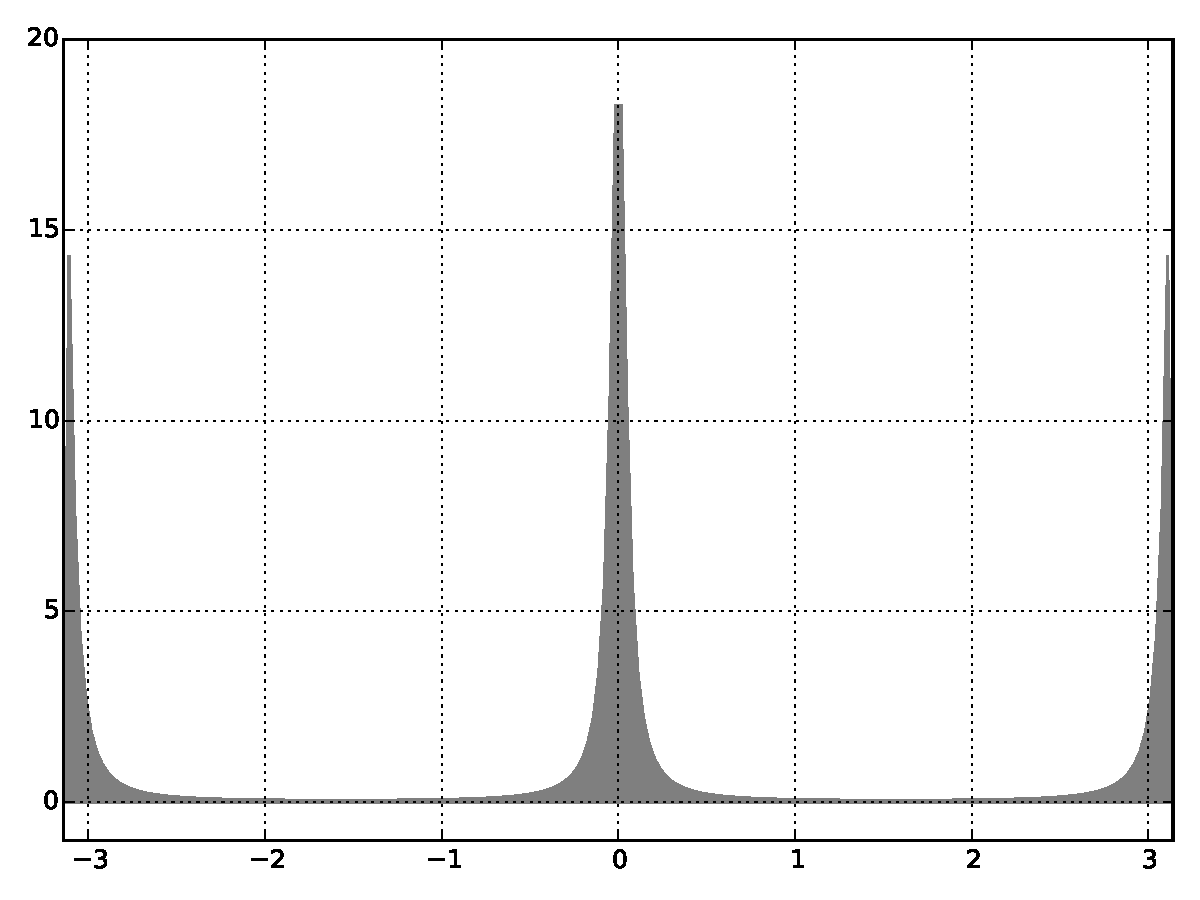
\includegraphics[width=0.9\textwidth]{./images/exact_1D.pdf}
		\caption{Exact}
		\label{fig:exact}
	\end{subfigure}
	\hspace*{-.65cm}
	\begin{subfigure}{0.36\textwidth}
		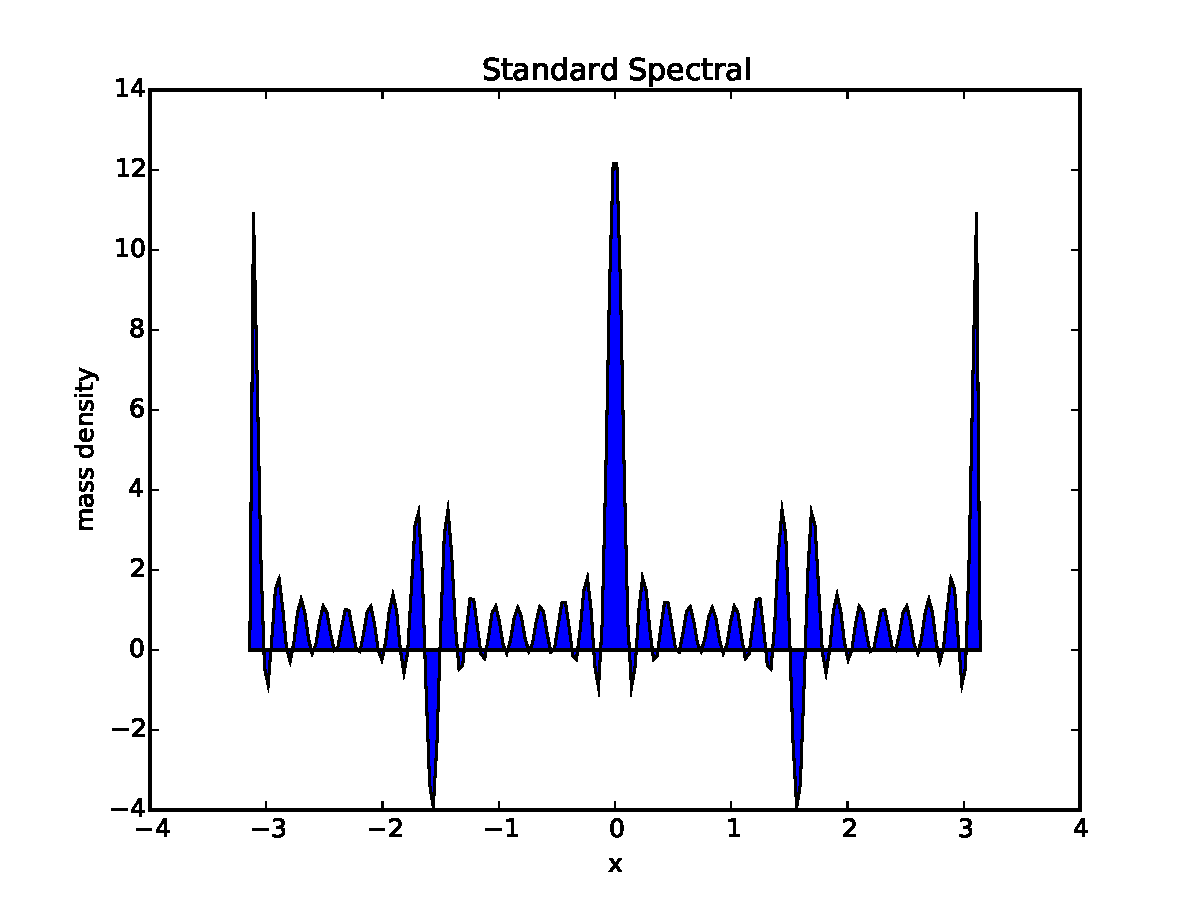
\includegraphics[width=0.9\textwidth]{./images/standard_spectral_1D.pdf}
		\caption{Standard spectral}
		\label{fig:standard spectral}
	\end{subfigure}
	\hspace*{-.65cm}
	\begin{subfigure}{0.36\textwidth}
		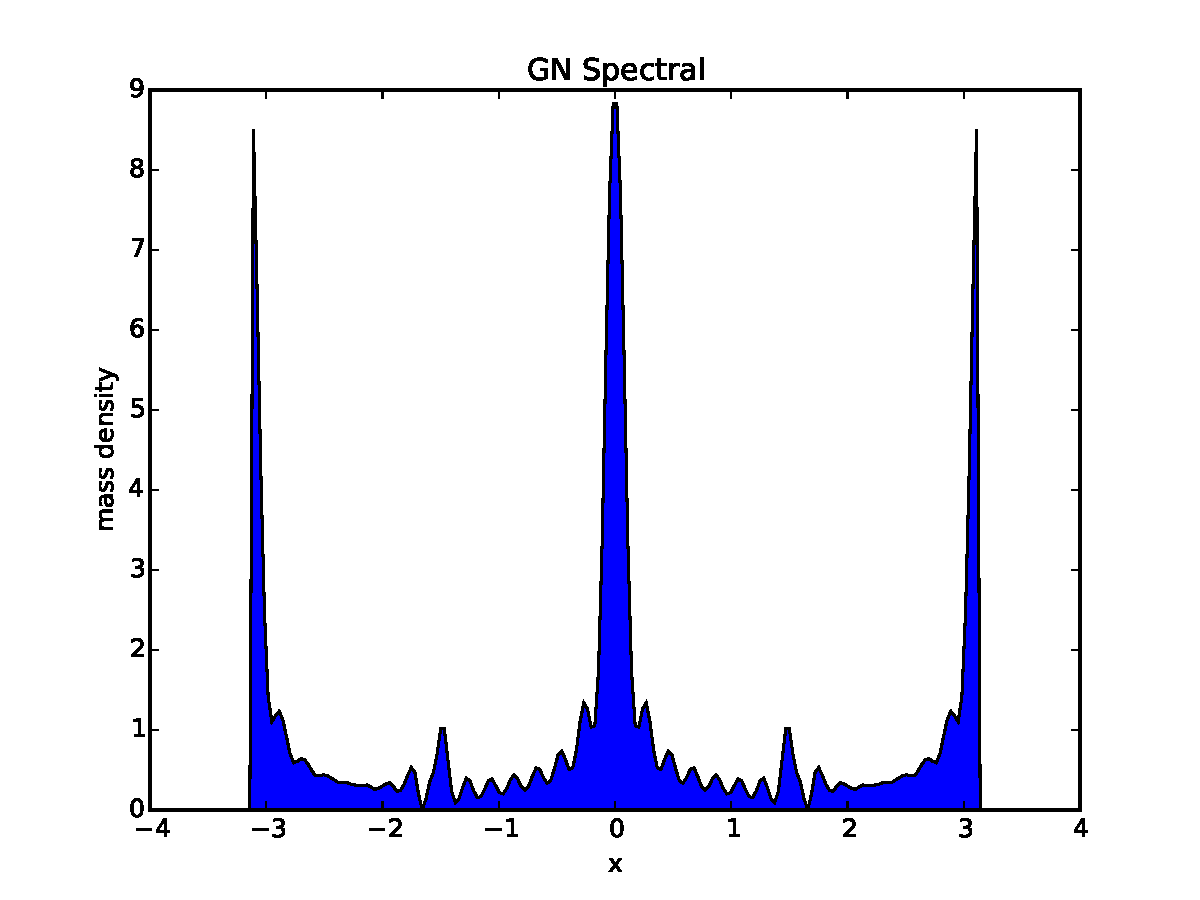
\includegraphics[width=0.9\textwidth]{./images/gn_spectral_1D.pdf}
		\caption{Algorithm \ref{alg:density}}
		\label{fig:gn spectral}
	\end{subfigure}
	\caption{A benchmark illustration of Algorithm \ref{alg:density} on the example described in Section \ref{sec:benchmark}.}
	\label{fig:S1}
\end{figure}

Here we witness how Algorithm \ref{alg:density} has greater qualitative accuracy than a standard spectral discretization, in the ``soft'' sense of qualitative accuracy.
For example, standard spectral discretization exhibits negative mass, which is not achievable in the exact system.
Moreover, the $L^{1}$-norm is not conserved in standard spectral discretization.  
In contrast, Theorem \ref{thm:norms} proves that the $L^{1}$-norm is conserved by Algorithm \ref{alg:density}.
A plot of the $L^{1}$-norm is given in Figure \ref{fig:L1}.
Finally, a convergence plot is depicted in Figure \ref{fig:convergence}.  
Note the spectral convergence of Algorithm \ref{alg:density}.
In terms of numerical accuracy, Algorithm \ref{alg:density} appears to perform better than a standard spectral method by a constant factor over a range of resolutions.

\begin{figure}
	\hspace*{-1.2cm}
	\centering
	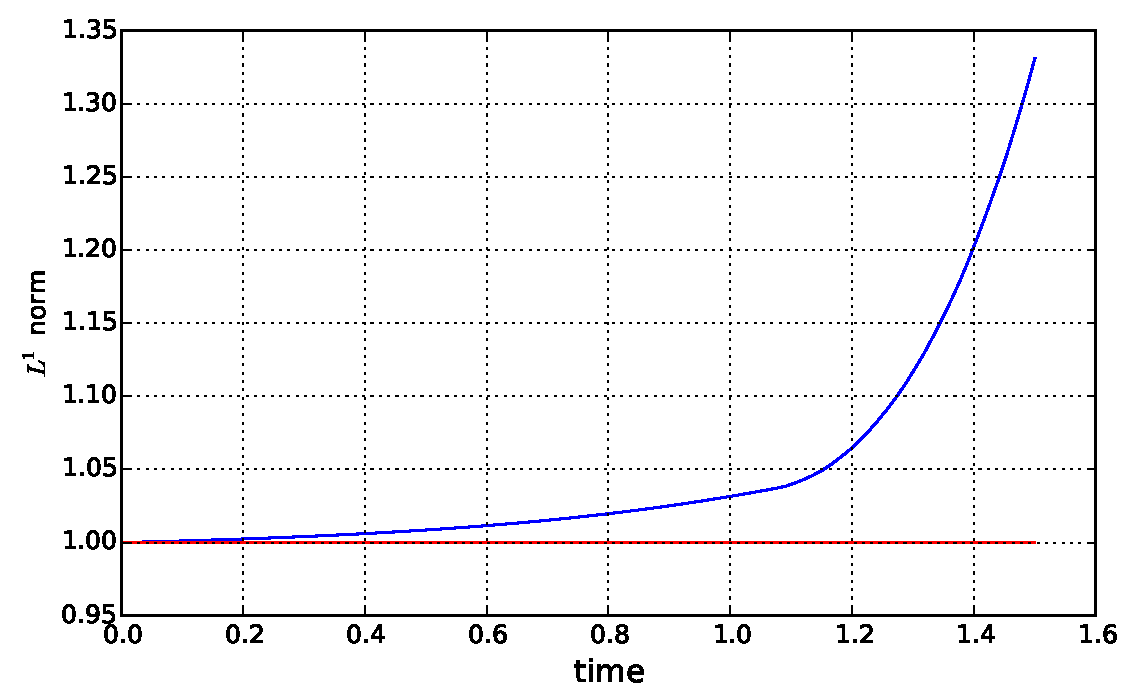
\includegraphics[width=\textwidth]{./images/L1_plot.pdf}
	\caption{A plot of the $L^{1}$-norm vs time of a standard spectral discretization (blue) and the result of Algorithm \ref{alg:density} (red) on the example described in Section \ref{sec:benchmark}.}
	\label{fig:L1}
\end{figure}

\begin{figure}
	\hspace*{-1.2cm}
	\centering
	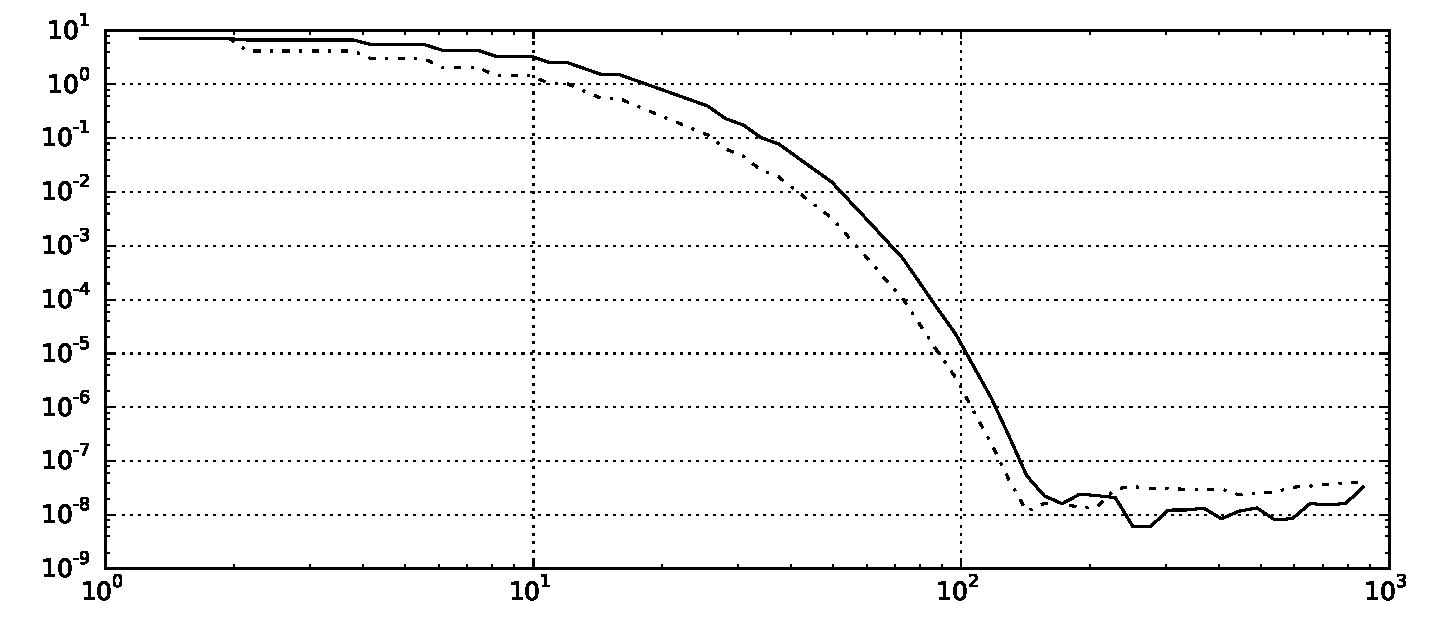
\includegraphics[width=0.9\textwidth]{./images/convergence_plot.pdf}
	\caption{Convergence plot for Algorithm \ref{alg:density} (red) and a standard spectral method (blue) in the $L^{1}$-norm.}
	\label{fig:convergence}
\end{figure}

%While a Fourier basis is convenient due to our ability to leverage existing fast Fourier transform packages, it is notable that we may use other basis.
%In particular, if we consider Daubechies wavelets with mother wavelet that have $4$ vanishing moments, then we may obtain solutions with much greater
%accuracy with fewer degrees of freedom. \todo[inline]{Ram should elaborate on this and include some pics.}
%At low resolutions, wavelet based solutions come at some cost in terms of sparsity, but this cost vanishes for large resolutions.
%
%\begin{figure}[h]
%	\centering
%	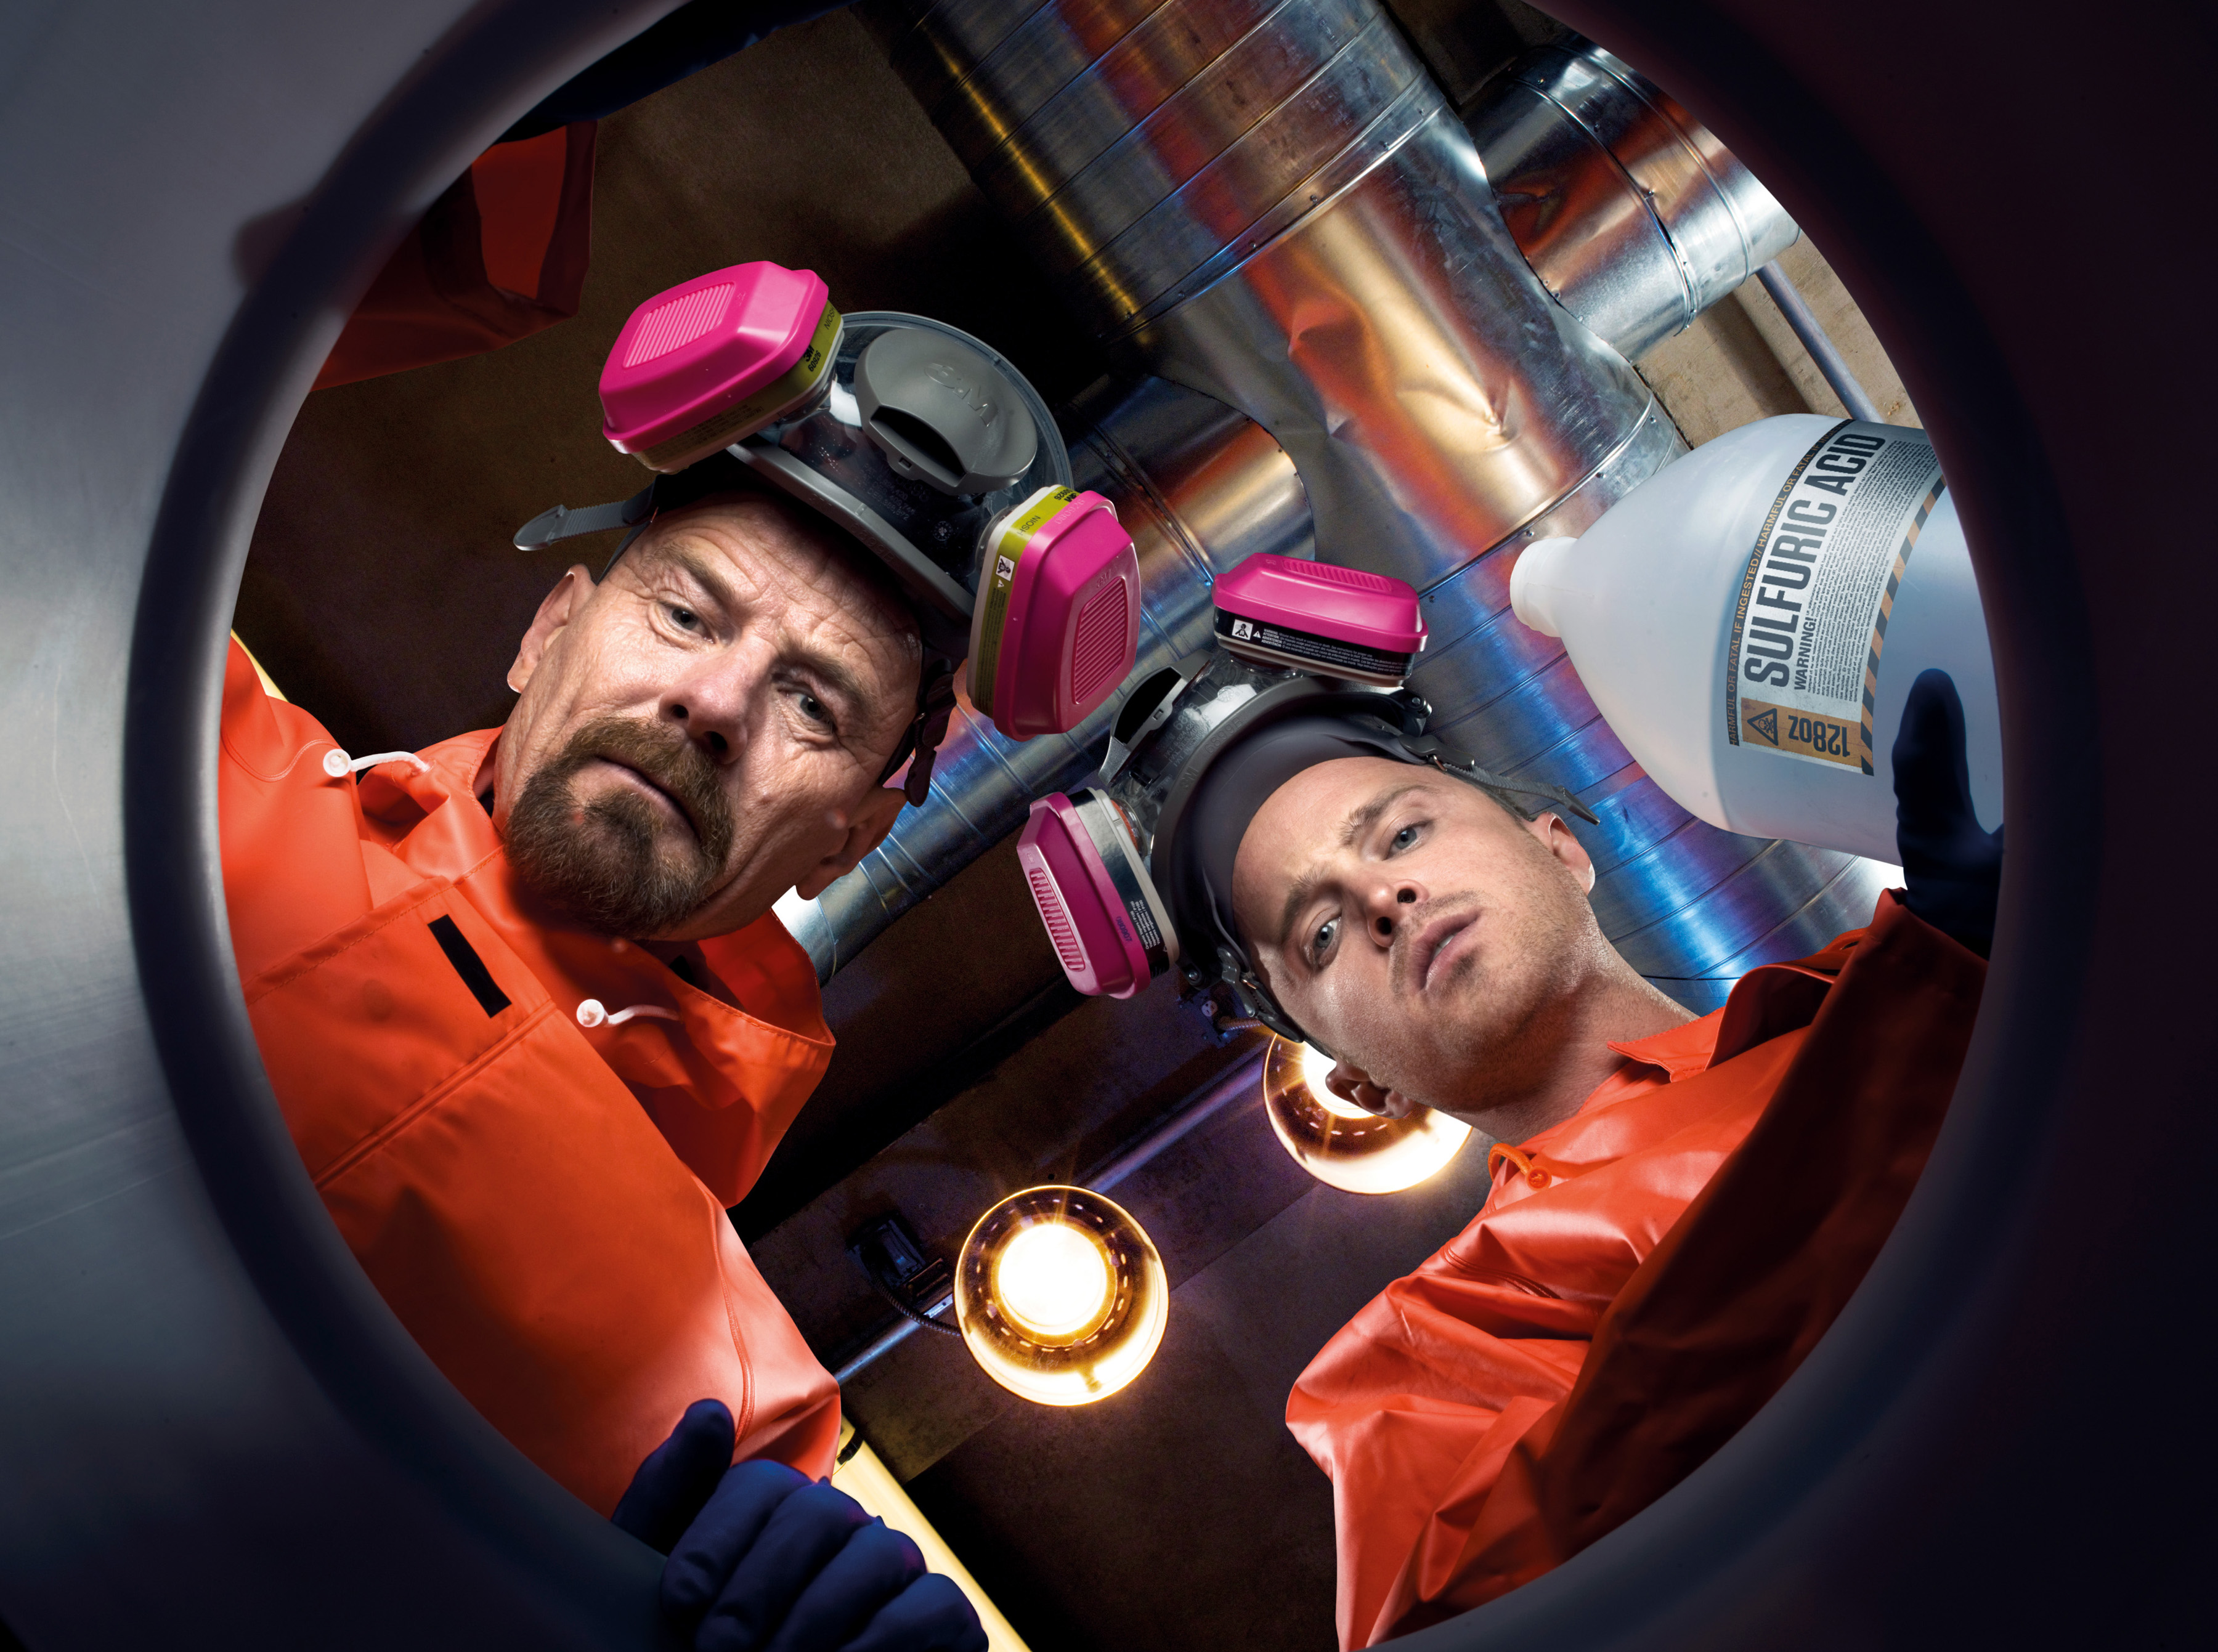
\includegraphics[width=0.2\textwidth]{./images/placeholder}
%	\caption{Algorithm \ref{alg:density} in a wavelet basis}
%\end{figure}


%To plot the output of Algorithm \ref{alg:function}, we must represent the operator $\hat{f}_{n}$ spectrally.
%The exact solution, $\hat{f}$, is represented via the Spectral Theorem \ram{citation} by considering its level sets.
%In the discrete case, we use the same representation for the purpose of plotting.
%An eigenvector-eigenvalue pair $(\lambda , \psi_{\lambda})$ is an approximation of the $\lambda$th level-set of $f$ by the density $\psi_{\lambda}^{2}$.
%\ram{this next portion of the discussion where the Gaussian smoothing is incorporated is adhoc. I understand that the results are not well defined, but why is Gaussian smoothing the right thing to show? It seems better discussion to ignore plotting and instead just speak about the tractability of the algorithm on functions and then the discussion on the Banach algebra.}
%In order to produce a reasonable output though these eigenvectors must be smoothed (they are not even well defined elements of $L^{2}(M)$ let alone $H^{1}$ in the high-resolution limit)
%We implement Algorithm \ref{alg:function} and plot with this in mind in Figure \ref{fig:quantum function 1} with respect to the initial condition $f_{0}(x) = \sin(x)$ and final time $t=1.5$.
%We have used a Gaussian smoothing of $\sigma=0.1$ in Figure \ref{fig:quantum 1}.
%The exact solution is given by 
%\begin{align}
%	f(x;t) = e^{2t} \sin(x) \left( \cos^{2}(x) + e^{4t} \sin^{2}(x) \right)^{-1/2},
%\end{align}
%and is plotted in \ref{fig:exact function 1}.
%Finally the result of using a standard spectral scheme is depicted in figure \ref{fig:standard function 1}.
%
%\begin{figure}[h]
%	\centering
%	\begin{subfigure}{0.3\textwidth}
%		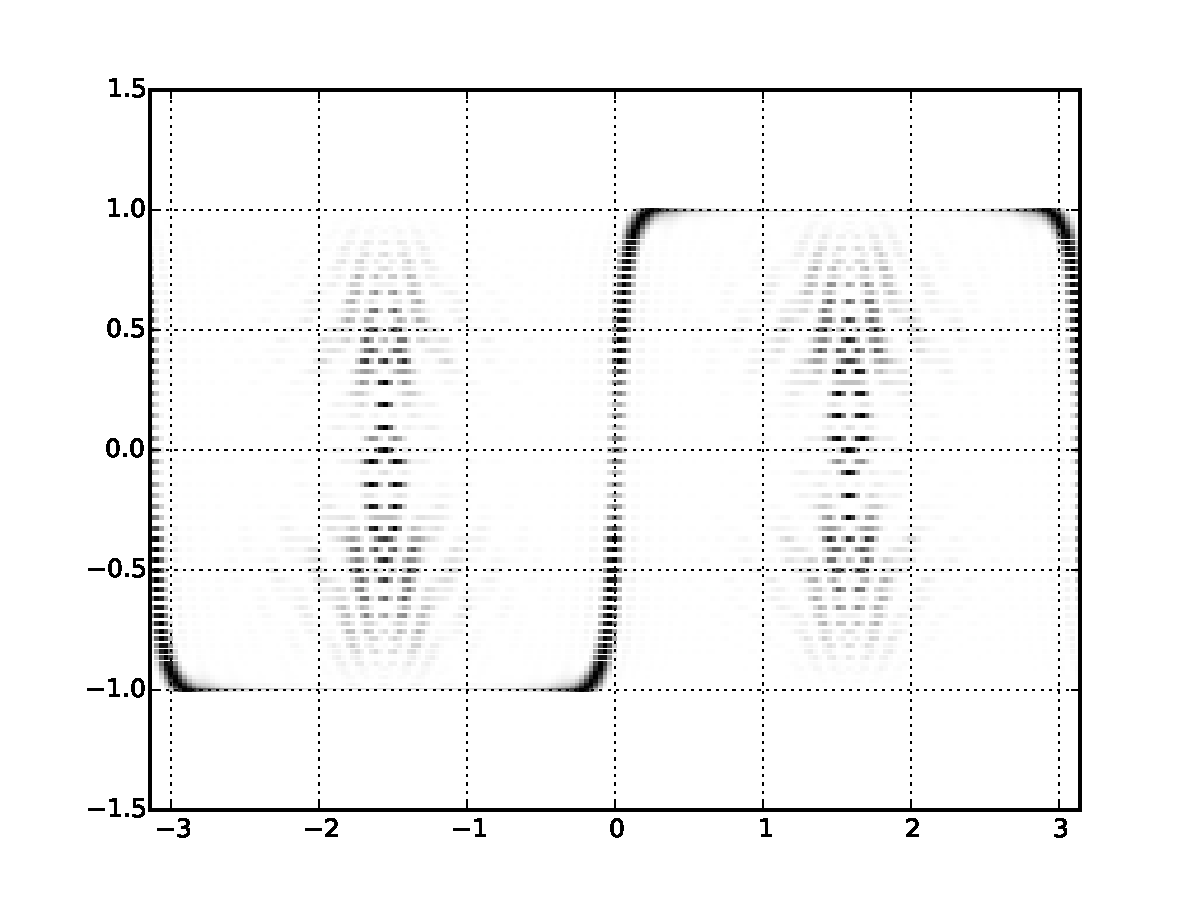
\includegraphics[width=\textwidth]{./images/function_plots/quantum_1.pdf}
%		\caption{Algorithm \ref{alg:function}}
%		\label{fig:quantum function 1}
%	\end{subfigure}
%	\begin{subfigure}{0.3\textwidth}
%		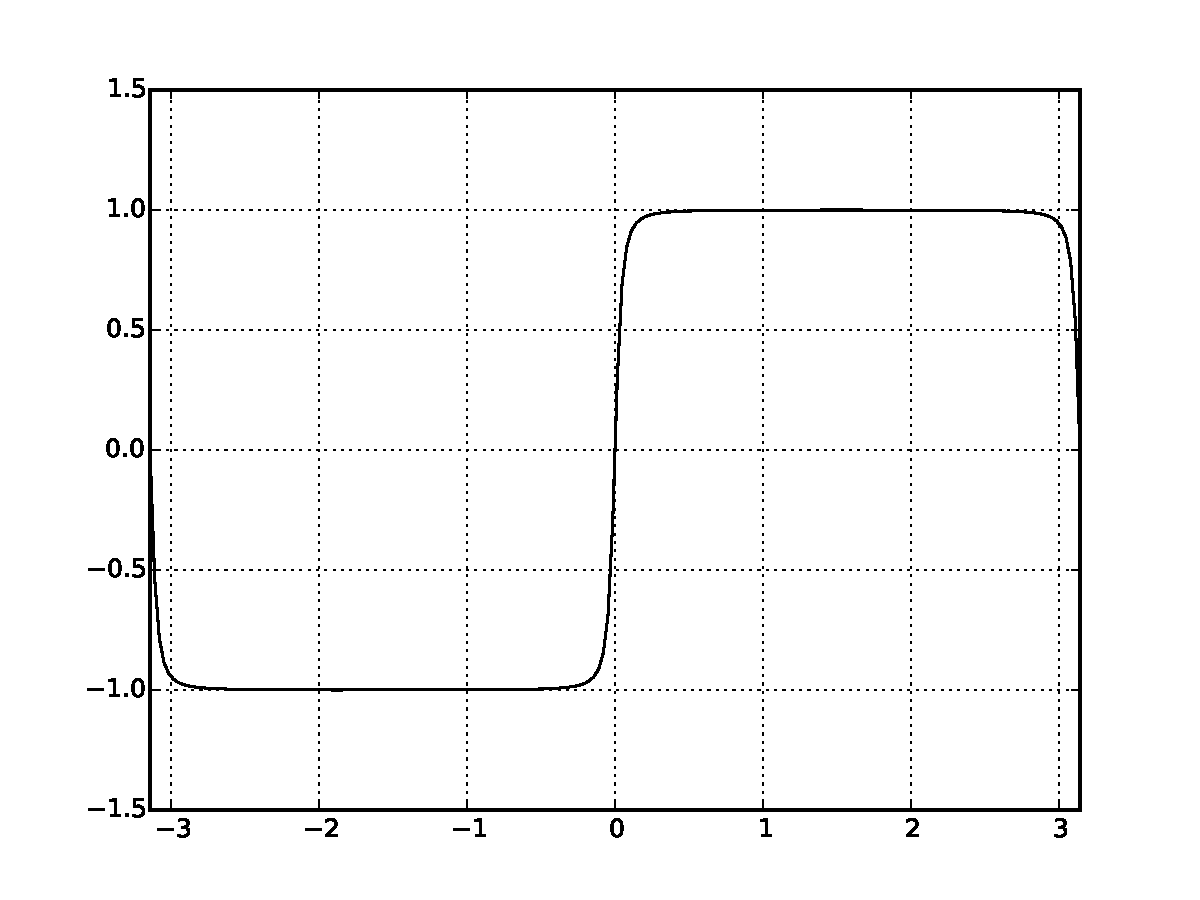
\includegraphics[width=\textwidth]{./images/function_plots/exact_1.pdf}
%		\caption{Exact solution}
%		\label{fig:exact function 1}
%	\end{subfigure}
%	\begin{subfigure}{0.3\textwidth}
%		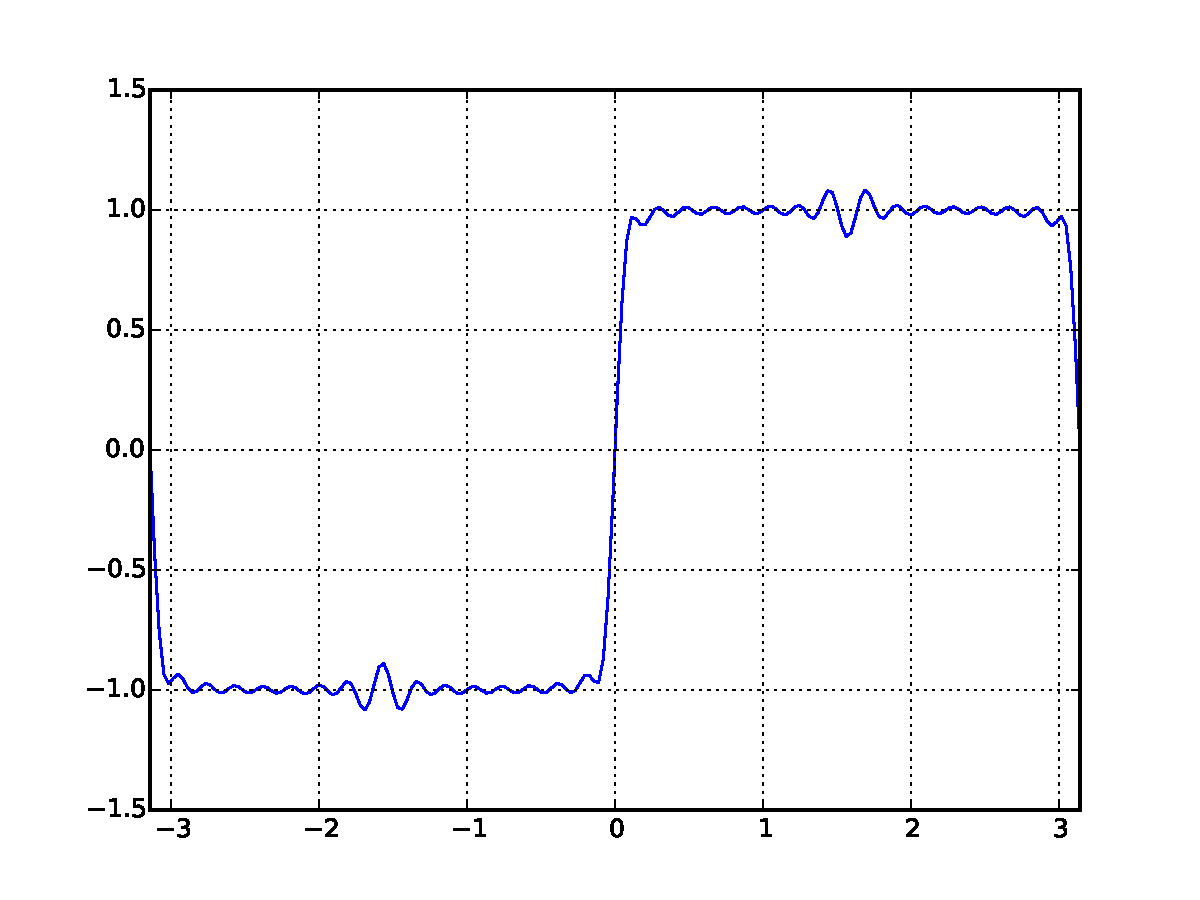
\includegraphics[width=\textwidth]{./images/function_plots/Koopman_1.pdf}
%		\caption{Standard spectral}
%		\label{fig:standard function 1}
%	\end{subfigure}
%	\caption{Solutions to \eqref{eq:function pde}}
%	\label{fig:function}
%\end{figure}
%
%From these plots it is unclear whether Algorithm \ref{alg:function} is more accurate than a standard spectral discretization.
%This is particularly problematic given the high cost of computation for Algorithm \ref{alg:function}  ($O(n^{2})$) versus a stand spectral computation ($O(n)$).
In general, Algorithm \ref{alg:function} is very difficult to work with, as it outputs an operator rather than a classical function.
However, Algorithm \ref{alg:function} is of theoretical value, in that it may inspire new ways of discretization (in particular, if one is only interested in a few level sets).
We will not investigate the potential of \ref{alg:function} to inspire other algorithms in this article, in the interest of focusing on the qualitative aspects of this discretization.
For example, under the initial conditions $g_{0}(x) = \cos(x)$ and $f_{0} = \sin(x)$ the exact solutions to \eqref{eq:quantum observable ode} are:
\begin{align*}
	g(x,t) &= \cos(x) \left( e^{4t} \sin^{2}(x) + \cos^{2}(x) \right)^{-1/2}\\
	f(x,t) &= \sin(x) \left( \sin^{2}(x) + e^{-4t} \cos^{2}(x) \right)^{-1/2}
\end{align*}
Under the initial condition $h_{0} = f_{0} \cdot g_{0}  = \sin(x) \cos(x)$ the exact solution to \eqref{eq:quantum observable ode} is:
\begin{align*}
	h(x,t) = f(x,t) g(x,t) = \cos(x) \sin(x) \left( \cos^{2}(x) + e^{4t} \sin^{2}(x) \right)^{-1}.
\end{align*}
One can compute $h$ by first multiplying the initial conditions and then using Algorithm \ref{alg:function} to evolve in time, or we may evolve each initial condition in time first, and multiply the outputs.
If one uses Algorithm \ref{alg:function}, then both options, as a result of Theorem \ref{thm:algebra}, yield the same result up to time discretization error (which is obtained with error tolerance $1e-8$ in our code).
In contrast, if one uses a standard spectral discretization, then these options yield different results with a discrepancy.
This discrepancy between the order of operations for both discretization methods is depicted in Figure \ref{fig:discrepancy}.

Finally, the sup-norm is preserved by the solution of \eqref{eq:function pde} \ram{citation}.
As shown in Theorem \ref{thm:quantize}, the sup-norm is equivalent to the operator norm when the functions are represented as operators on $L^{2}(M)$.
As proven by Theorem \ref{thm:norms}, the operator-norm is conserved by Algorithm \ref{alg:function}.
In contrast, the sup-norm drifts over time under a standard discretization.  
This is depicted in Figure \ref{fig:norms}

\begin{figure}[h]
	\hspace*{-1.2cm}
	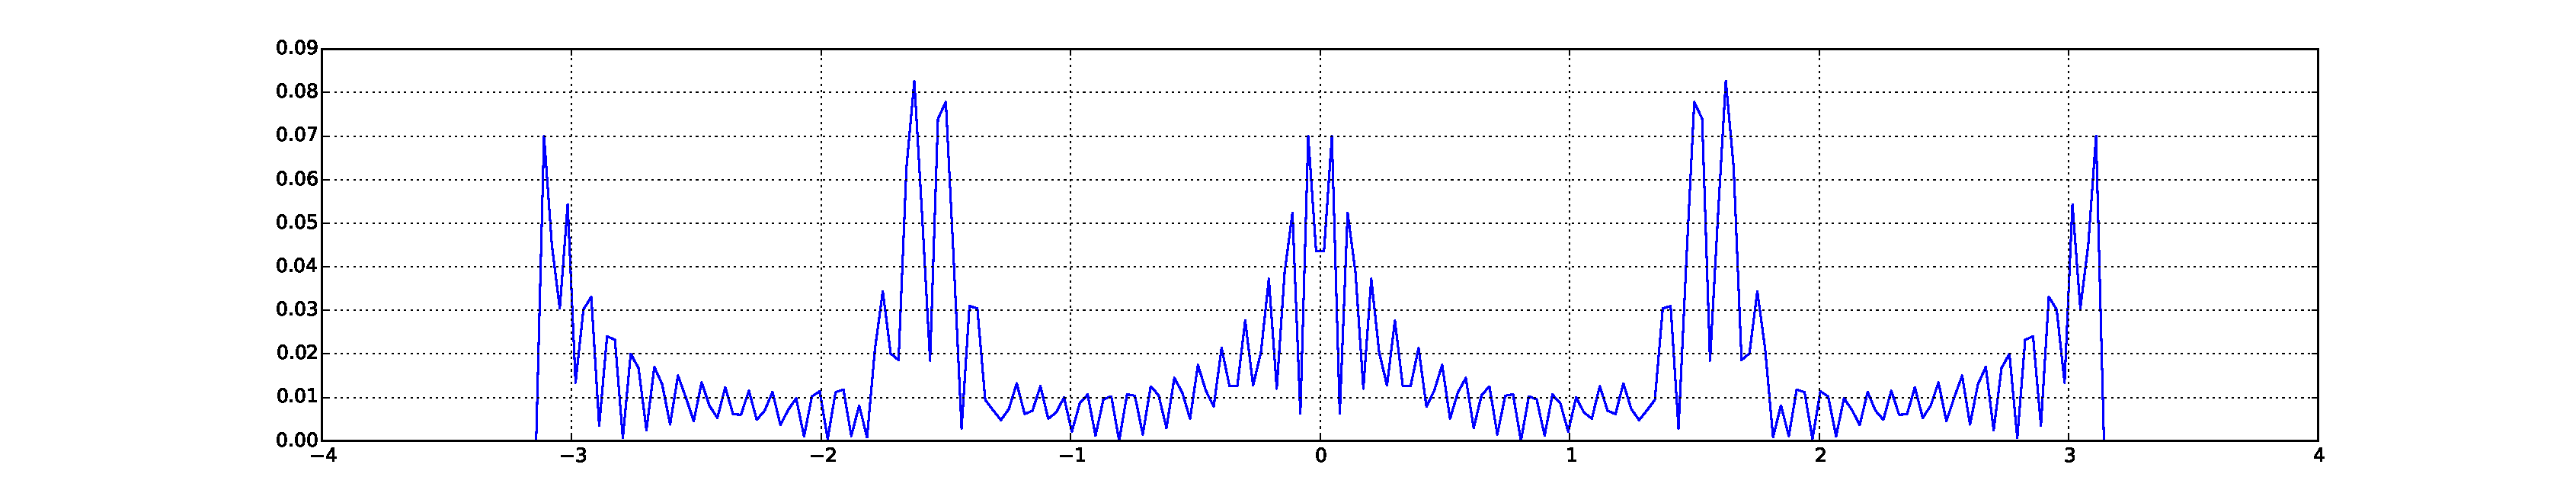
\includegraphics[width=1.15\textwidth]{./images/function_plots/discrepancy}
	\caption{The discrepancy due to non-preservation of scalar products under a standard spectral discretization (blue) and under the discretization described in Algorithm \ref{alg:function} (red). 
	Note that the discrepancy due to Algorithm \ref{alg:function} is difficult to see because it is of order $10^{-8}$. \ram{why not use a logarithmic plot? Also could you label the axes?} }
	\label{fig:discrepancy}
\end{figure}  

\begin{figure}[h]
	\hspace*{-1.2cm}
	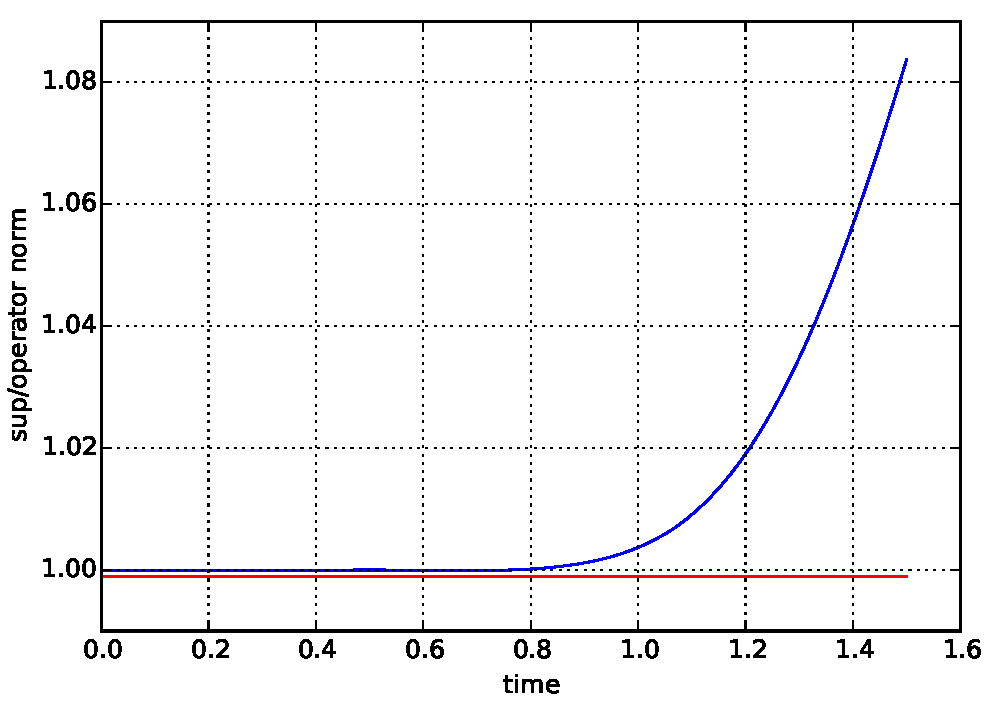
\includegraphics[width=1.15\textwidth]{./images/L_inf_plot.pdf}
	\caption{A plot of the sup-norm vs time of a standard spectral discretization (blue) and the result of Algorithm \ref{alg:function} (green) on the example described in Section \ref{sec:benchmark}. \ram{can you label the x-axis and make the markings larger since it is hard to see them now. Also it would probably be useful if you kept the color consistent throughout (blue for standard discretization and red for our methods)}}
	\label{fig:norms}
\end{figure}
%However, we can obtain one estimate by applying $\hat{f}_{n}$ to the half-density $\sqrt{dx}$, and then divide the result by $\sqrt{dx}$.
%The resulting function appears to approximate $f(x;t)$ well in the flat areas, and overshoot at the peaks.
%In comparison, a standard spectral discretization seems to have large spurious oscillations in the center.
%These estimates are plotted alongside the exact solution in figure \ref{fig:function}.
%We should note that our means of converting $\hat{f}_{n}$ into a function is probably not the best choice of a left inverse to the hat-map.
%Different choices yield different approximations to $f(x;t)$, some
%of which get the peaks correct, but do poorly in the valleys.
%\begin{figure}[h!]
%	\centering
%	\begin{subfigure}{0.4\textwidth}
%		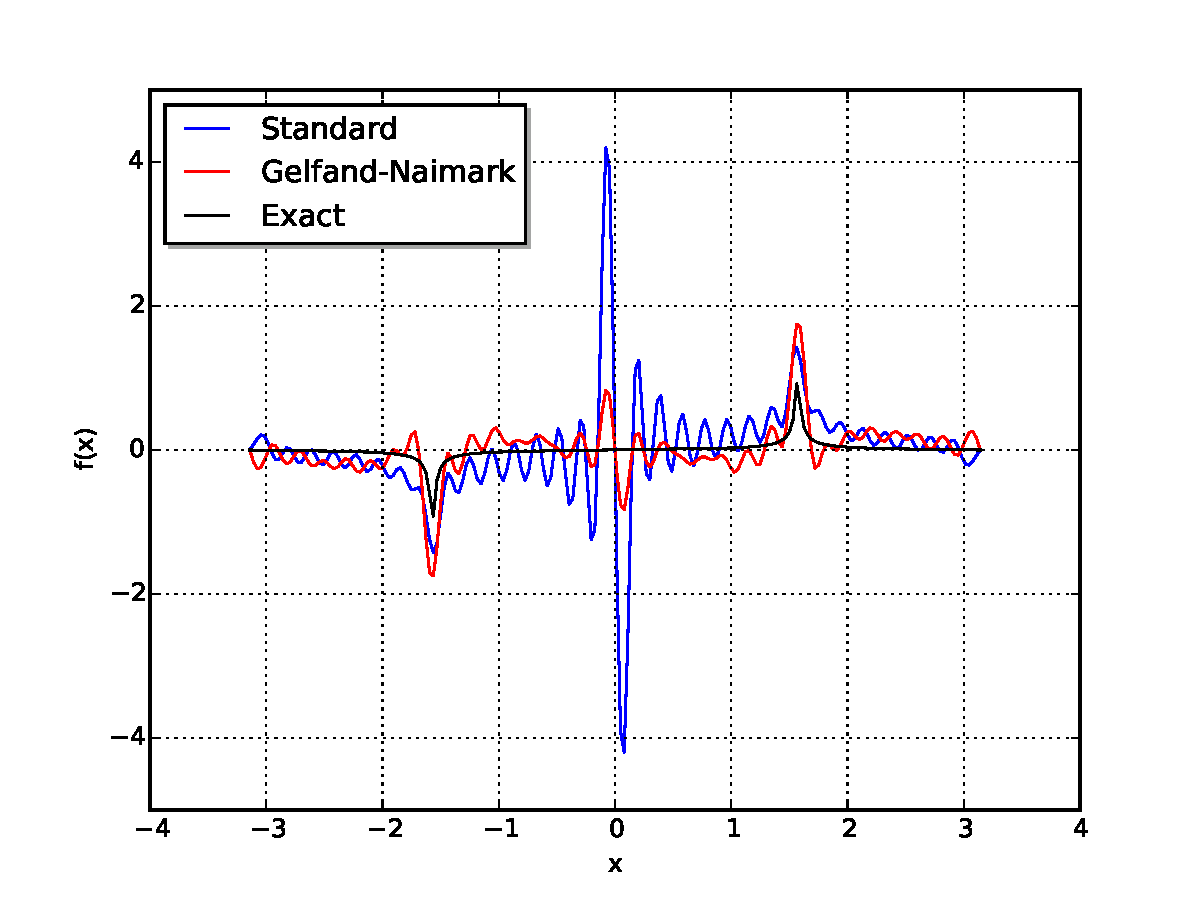
\includegraphics[width=\textwidth]{./images/function_comparison.pdf}
%		\caption{Functions}
%		\label{fig:function}
%	\end{subfigure}
%	\begin{subfigure}{0.4\textwidth}
%		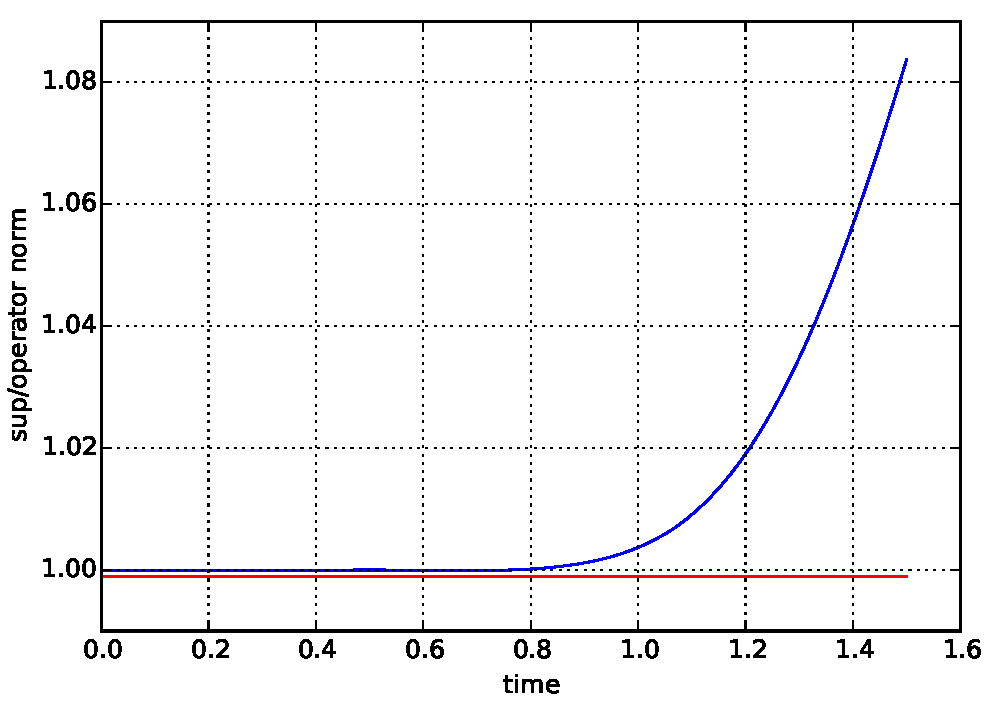
\includegraphics[width=\textwidth]{./images/L_inf_plot.pdf}
%		\caption{Operator norms}s
%		\label{fig:sup norm}
%	\end{subfigure}
%	\caption{Numerical results for a one-dimensional system}
%\end{figure}


%\subsection{A system on the 2-torus}
%Let us consider the system on $\mathbb{T}^{2}$ given by 
%\begin{align}
%	\dot{x} &= \cos(2\pi y) - D \sin(2\pi x) \\
%	\dot{y} &= -\sin(2 \pi x) - D \cos(2 \pi y).
%\end{align}
%This can be seen as a dissipative Hamiltonian system with Hamiltonian $H(x,y) = \sin(2 \pi y) - \cos(2 \pi x)$ and dissipation $\vec{F} = D \cdot \nabla H$.
%When $D=0$, we have an integrable system and volume is preserved with respect to the standard volume form on $\mathbb{T}^{2}$.
%When $D>0$ the system exhibits phase space contraction near minima of $H$ and phase space expansion near the maxima of $H$.
%In particular, there are four equilibria:
%\begin{center}
%\begin{tabular}{cc}
%	$(x,y)$ & Type \\
%	\hline
%	$(0, 1/4)$ & saddle \\
%	$(0, 3/4)$ & sink with clockwise rotation\\
%	$(1/2,1/4)$ & source with counter-clockwise rotation \\
%	$(1/2,3/4)$ & saddle
%\end{tabular}
%\end{center}
%
%If we place a wrapped Guassian probability distribution with center at $(\bar{x},\bar{y}) = (0.4,0.4)$ and variance $\sigma = 0.3$ we should expect much of the mass to be swept by the unstable
%axis of the saddle at $(0,1/4)$ and sucked towards the sink at $(0,3/4)$.
%In Figure \ref{fig:2 torus} we depict the result of solving \eqref{eq:density pde} using three methods: Algorithm \ref{alg:density}, Monte-Carlo, and a standard spectral discretization.
%The top row depicts the result from applying algorithm 2 with the Fourier basis $\{ e^{2\pi i (k_{1}x +k_{2}y)} \mid -8 \leq k_{1},k_{2} \leq 8\}$.
%This is a total of $289$ basis functions. 
%The middle row depicts the results of a Monte-Carlo simulation with $10^{5}$ particles.
%Finally, the bottom row depicts the results of a standard spectral scheme using the same basis as mentioned earlier.
%The Monte-Carlo simulation can serve us as a benchmark.
%We see that spurious oscillations will manifest using standard discretization, just as in the one-dimensional case.
%Also as before, our Algorithm \ref{alg:density} will conserve mass while the standard spectral scheme will diffuse and even negate mass.
%By inspection, it appears the largest unstable mode of the standard spectral algorithm is a function with rapid spatial oscillations.
%The dominance of this function can be seen visually at time $0.6$ in figure \ref{fig:2 torus}.
%
%\begin{figure}[h!]
%	\centering
%	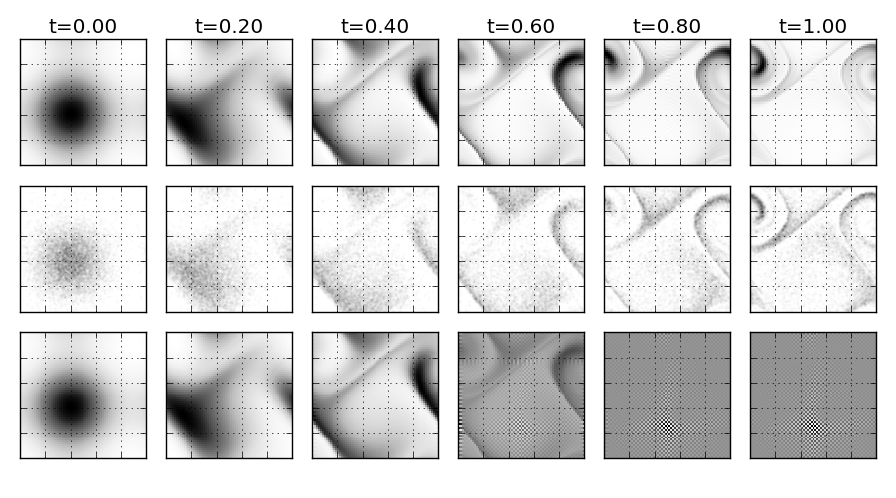
\includegraphics[width=0.8\textwidth]{./images/two_torus.png}
%	\caption{ \tiny {\bf Top:} Algorithm \ref{alg:density}, {\bf Middle:} Monte Carlo, {\bf Bottom:} Standard Spectral}
%	\label{fig:2 torus}
%\end{figure}

%Even at dimension $d=2$ Algorithm \ref{alg:function} becomes troublesome, although still feasible.
%Instead we implement a particle method based upon the method of characteristics.
%Using the initial function $f_{0}(x,y) = \sin(2\pi y)$ we observe the numerical results shown in Figure \ref{fig:particle function}
%
%\begin{figure}[h!]
%	\centering
%	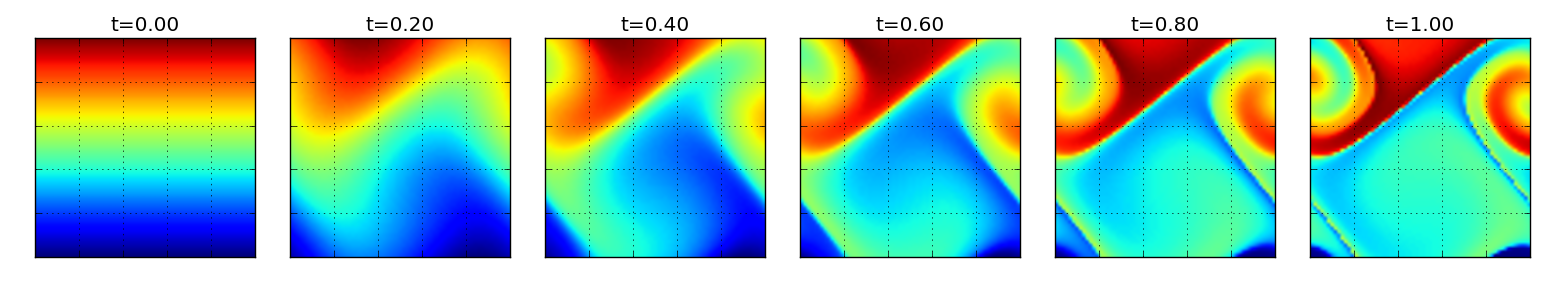
\includegraphics[width=0.7\textwidth]{./images/psuedo_spec_Koopman.png}
%	\caption{The result of a particle method with initial condition $f_{0}(x,y) = \sin(2\pi y)$.}
%	\label{fig:particle function}
%\end{figure}
%
%We can take the inner-product of a density the function output by our respective algorithms.
%This inner-product is constant in time for exact solutions to the pdes.
%For our numerical solutions these inner-products drift.
%However, there is substantially greater drift and variation when using a standard spectral discretization.
%These results are shown in Figure \ref{fig:inner}. 
%\begin{figure}[h!]
%	\centering
%	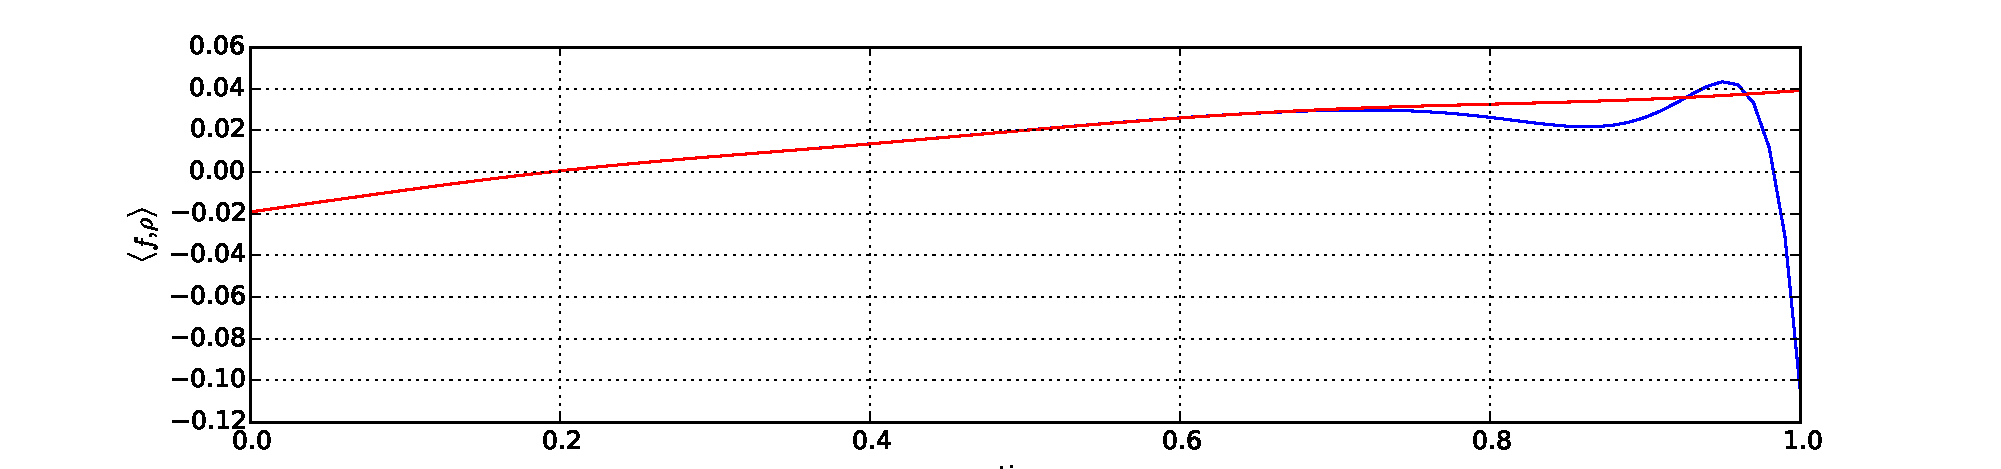
\includegraphics[width=0.7\textwidth]{./images/inner_product_plot.pdf}
%	\caption{The inner product between numerically densities and functions.  Blue depicts standard spectral discretization, red depicts the results from Algorithm \ref{alg:density}.}
%	\label{fig:inner}
%\end{figure}


\subsection{A modified ABC flow}
\label{sec:ABC_flow}

Consider the system
\begin{align}
	\dot{x} = A \sin( 2\pi z) + C \cos(2\pi y)  + D \cos(2\pi x)\\
	\dot{y} = B \sin( 2\pi z) + A \cos(2\pi y)  + D \cos(2\pi y)\\
	\dot{z} = A \sin( 2\pi z) + B \cos(2\pi y)  + D \cos(2\pi z)
\end{align}
on the three-torus for constants $A,B,C,D \in \mathbb{R}$.  
When $D=0$ this system is the well studied volume conserving system known as an Arnold-Beltrami-Childress flow \ram{citation}.
When $A > B > C > 0$, $D=0$, and $C << 1$, then the solutions to this ODE are chaotic, with a uniform steady state distribution \cite{MajdaBertozzi2002}.
When $D=0$ the operator $\pounds_{X}$ of \eqref{eq:half density pde} is identical to the operator $\partial_{\alpha}( \rho X^{\alpha})$ that appears in \eqref{eq:density pde}, and Algorithm \ref{alg:half density} will not differ from a standard spectral discretization.\footnote{This is always the case for a volume conserving system.}
Therefore we consider the case where $D > 0$ to see how our discretization are differs from the standard one.
When $D> 0$ volume is no longer conserved and there is a non-uniform steady-state distribution.

%Given any probability distribution on $\mathbb{R}^{3}$ we can get a probability distribution on $\mathbb{T}^{3}$ by wrapping it around.
%That is to say for any $p \in L^{1}(\mathbb{R}^{3})$ we can consider the probability distribution on $\tilde{p} \in L^{1}(\mathbb{T}^{3})$ implicitly given by
%\begin{align*}
%	\int_{A} \tilde{p}( {\bf x} ) = \sum_{ {\bf k} \in \mathbb{Z}^{3} } \int_{A + {\bf k} } p( {\bf x} + {\bf k} ).
%\end{align*}
%for any Borel set $A \subset \mathbb{T}^{3}$ where we view $\mathbb{T}^{3}$ as a unit-cube with boundaries identified.
%
%In particular, let
%\begin{align}
%	p(x,y,z) = \frac{1}{ (\sigma_{x} \sigma_{y} \sigma_{z} )\sqrt{ 2\pi } } e^{ - \frac{1}{2} ( (x/\sigma_{x})^{2} + (y/\sigma_{y})^{2} +  (z/\sigma_{z})^{2} )}
%\end{align}
%with $\sigma_{x} = 0.2, \sigma_{y} = 0.3, \sigma_{z} = 0.3$.
For the following numerical experiment let $A=1.0,B=0.5,C=0.2,$ and $D=0.5$.
As an initial condition consider a wrapped Gaussian distribution with anisotropic variance $\sigma= (0.2, 0.3, 0.3)$ centered at $(0,0,0)$.
Equation \eqref{eq:density pde} is approximately solved using Algorithm \ref{alg:density}, Monte-Carlo, and a standard spectral method.
The results of the $z$-marginal of these densities are illustrated in Figure \ref{fig:ABCD}.
The top row depicts the results from using Algorithm \ref{alg:density} using $33$ modes along each dimension.
The middle row depicts the results from using a Monte-Carlo method with $15^{3} = 3375$ particles as a benchmark computation.
Finally, the bottom row depicts the results from using a standard Fourier based discretization of \eqref{eq:density pde} using 33 modes along each dimension.
Notice that Algorithm \ref{alg:density} performs well when compared to the standard discretization approach.

\begin{figure}
	\centering
	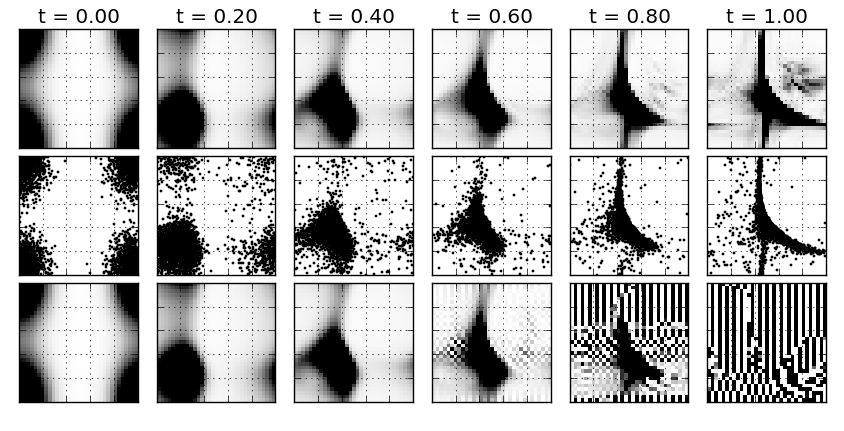
\includegraphics[width=1\textwidth]{./images/ABCD_flow.png}
	\caption{An illustration of the performance of Algorithm \ref{alg:density} (top row), Monte Carlo (middle row) and a standard spectral approach (bottom row) on the example described in Section \ref{sec:ABC_flow} \ram{what does black and white represent? Also it would be useful to label the x axes of the bottom row and the y axes of the left column}}
	\label{fig:ABCD}
\end{figure}

%\section{Future work}
%There are a number of areas to consider for future research.  We propose the following:
%
%\subsection{Relaxing assumptions on $M$}
%In this paper we have assumed $M$ to be a compact manifold without boundary.
%While this provides a good starting point, the most common domains in engineering are various cartesian products of the unit interval, $[0,1]$ and $\mathbb{R}^{n}$.
%
%In the case where $M$ is compact with boundary, the methods described here can be imported without change as long as the vector field is tangential or vanishing on the boundary.
%However, when $X$ is transverse to the boundary of $M$, then we must find a way of dealing with flux.
%
%In the case $M = \mathbb{R}$, the primary issue is that $L^{2}(\mathbb{R})$ is not a separable Hilbert space.
%In order to handle such a scenario a sacrifice must be paid.  Perhaps we should resign ourselves to seek convergence on a subspace of $L^{2}(\mathbb{R})$.
%This can be done by using a basis, such as Hermite functions $\{ H_{n}(x) \exp^{-x^{2}/2}\}$ where $H_{n}(x)$ is the $n$th physicists polynomial.
%In this case we would be converging on the separable subspace $L^{2}( \mathbb{R};  w)$ where where the $L^{2}$-inner product is taken with respect to the weight function $w = \exp( -x^{2})$.
%
%\subsection{Systems with noise}
%The PDEs \eqref{eq:function pde} and \eqref{eq:density pde} can be seen as zero-noise limits of Kolmogorov equations (a.k.a. Fokker Plank equations, a.k.a. Master equations).
%When noise is added, equations \eqref{eq:function pde} and \eqref{eq:density pde} become
%\begin{align*}
%	\partial_{t} f + X^{i} \partial_{i} f = \Delta f \\
%	\partial_{t} \rho + \partial_{i} ( \rho X^{i}) = \Delta \rho
%\end{align*}
%
%In order to address such a change, we need to understand first how half-density are affected.
%It is easy to derive that an equation of the form
%\begin{align*}
%	\partial_{t} \psi + \frac{1}{2} X^{i} \partial_{i} \psi + \frac{1}{2} \partial_{i}( \psi X^{i} ) = D \cdot \psi
%\end{align*}
%where $D$ is any formal square root of $\Delta$ (i.e. a \emph{Dirac operator}).
%The approach of \cite{Crane2013} to discretize mean curvature flows by identifying ``mean-curvature modulo scaling'' as half-density could be a manifestation of this idea, but this has yet to be verified.
%

\section{Conclusion}

In this paper we constructed a numerical scheme for \eqref{eq:function pde} and \eqref{eq:density pde} that is spectrally convergent and qualitatively accurate, in the sense that natural invariants are preserved.
The result of obeying such conservation laws is a robustly well-behaved numerical scheme at a variety of resolutions where legacy spectral methods fail.
This claim was verified in a series of numerical experiments which directly compared our algorithms with standard Fourier spectral algorithms.
The importance of these conservation laws was addressed in a short discussion on the Gelfand Transform.
We found that conservation laws completely characterize \eqref{eq:function pde} and \eqref{eq:density pde}, and this explains the benefits of using qualitatively accurate scheme at a more fundamental level.


\subsection{Acknowledgements}
This paper developed over the course of years from discussions with many people whom we would like to thank: Jaap Eldering, Gary Froyland,
 	Darryl Holm, Peter Koltai, Stephen Marsland, Igor Mezic, Peter Michor, Dmitry Pavlov, Tilak Ratnanather, and Stefan Sommer. 
This research was made possible by funding from the University of Michigan.

%\appendix
%\section{A list of legacy algorithms}
%\label{app:algorithms}
%In this section we provide standard algorithms for solving \eqref{eq:function pde} and \eqref{eq:density pde}.
%The first algorithm we present is a particle method for solving \ref{eq:function pde} based upon the method of characteristics.
%
%\begin{algorithm}[h]
%	\KwData{An initial function $f_{0}$, a resolution $n \in \mathbb{N}$, and a final time $T>0$.}
%	\KwResult{The value of the solution $f(x,t)$ to \eqref{eq:function pde} at time $t=1$ at a finite set of points.}.
%	Initialize a set of points $\{ x_{1},\dots,x_{n} \}$ on $M$ (e.g. a regular grid) \;
%	\For{i = 1,\dots,n}{
%		Backward integrate the ode $\dot{x} = X(x)$ from final condition $x_{i}(T)$ using a method of choice (e.g. Euler's method) up to time $t=0$\;
%	}
%	\KwOut{ $f_{0}( x_{1}(0) ), \dots, f_{0}(x_{n}(0) )$. }
%	\caption{The method of characteristics}\label{alg:particle}
%\end{algorithm}
%
%A similar particle method can be used to solve \eqref{eq:density pde}.
%In essence this is possible because distributions form the dual space to functions, and \eqref{eq:density pde} is the dual evolution equation to \eqref{eq:function pde}.
%In the case where our density is a probability distribution, this algorithm is commonly referred to as a Monte Carlo method.
%
%\begin{algorithm}[h]
%	\KwData{An initial probability density $\rho_{0}$, a resolution $n \in \mathbb{N}$, and a final time $T>0$.}
%	\KwResult{An approximation of the solution $\rho(x,t)$ to \eqref{eq:desity pde} at time $t=1$ as a finite sum of Dirac delta distributions.}.
%	Initialize a set of points $\{ x_{1},\dots,x_{n} \}$ on $M$ by sampling the probability density $\rho_{0}$\;
%	\For{i = 1,\dots,n}{
%		Integrate the ode $\dot{x} = X(x)$ and the Jacobian matrix equation $\dot{J} = DX(x)\cdot J$ with the initial conditions $x_{i}$ using a method of choice (e.g. Euler's method) up to time $t=T$\;
%	}
%	\KwOut{ $\sum_{i} \frac{1}{\det(J)} \delta_{x_{i}(T)}$ where $\delta_{x}$ denotes the Dirac delta distribution centered at $x$. }
%	\caption{A Monte Carlo method}\label{alg:Monte Carlo}
%\end{algorithm}
%
%For vector-fields on the torus we can leverage Fast Fourier Transform libraries to represent \eqref{eq:function pde} and \eqref{eq:density pde} in the Fourier domain.
%In particular on the unit circle $S^{1}$ the vector-field $X$ is represented by a continuous function with a Fourier expansion $X(x) = \sum_{k=-\infty}^{\infty} \hat{X}_{k} \exp( 2\pi i kx)$.
%The PDEs \eqref{eq:function pde} and \eqref{eq:density pde} are then represented in the Fourier domain as
%ODEs on the Fourier coefficients
%\begin{align}
%	\frac{d \hat{f}_{k}}{dt} + 2\pi i \ell \hat{X}_{k-\ell} \hat{f}_{\ell} = 0 \\
%	\frac{d \hat{\rho}_{k}}{dt} + 2\pi i k \hat{X}_{k-\ell} \hat{f}_{\ell} = 0
%\end{align}
%where $\hat{f}_{k}$ and $\hat{\rho}_{k}$ represent the Fourier expansions of the solution to \eqref{eq:function pde} and \eqref{eq:density pde}.
%This inspires the following spectral methods.
%
%\begin{algorithm}[h]
%	\KwData{An initial density $\rho_{0}$, a resolution $n \in \mathbb{N}$, and a final time $T > 0$.}
%	\KwResult{A truncated Fourier series which approximates the solution $\rho(x,t)$ to \eqref{eq:density pde}, at time $t=T$.}
%	Compute the Fourier expansion of $X = \hat{X}_{k} \exp( 2\pi i k)$ for $k=-n,\dots,0,\dots,n$\;
%	Compute the Fourier expansion of $f_{0} = \hat{f}_{0,k} \exp( 2\pi i k)$ for $k=-n,\dots,0,\dots,n$\;
%	Solve a truncated version of the linear system \eqref{eq:standard spectral} up to time $t=1$.\;
%	\KwOut{$\hat{f}_{1,k}$ for $k= -n , \dots, 0 ,\dots,n$.}
%	\caption{A standard spectral method for \eqref{eq:density pde}}\label{alg:spectral density}
%\end{algorithm}
%
%\begin{algorithm}[h]
%	\KwData{An initial function $f_{0}$, a resolution $n \in \mathbb{N}$, and a final time $T > 0$.}
%	\KwResult{A truncated Fourier series which approximates the solution $f(x,t)$ to \eqref{eq:function pde}, at time $t=T$.}
%	Compute the Fourier expansion of $X = \hat{X}_{k} \exp( 2\pi i k)$ for $k=-n,\dots,0,\dots,n$\;
%	Compute the Fourier expansion of $f_{0} = \hat{f}_{0,k} \exp( 2\pi i k)$ for $k=-n,\dots,0,\dots,n$\;
%	Solve a truncated version of the linear system \eqref{eq:standard spectral} up to time $t=1$.\;
%	\KwOut{$\hat{f}_{1,k}$ for $k= -n , \dots, 0 ,\dots,n$.}
%	\caption{A standard spectral method for \eqref{eq:function pde}}\label{alg:spectral function}
%\end{algorithm}


\bibliographystyle{siam}
\bibliography{hoj.bib}
\end{document}
